\documentclass[]{article}
\usepackage{lmodern}
\usepackage{amssymb,amsmath}
\usepackage{ifxetex,ifluatex}
\usepackage{fixltx2e} % provides \textsubscript
\ifnum 0\ifxetex 1\fi\ifluatex 1\fi=0 % if pdftex
  \usepackage[T1]{fontenc}
  \usepackage[utf8]{inputenc}
\else % if luatex or xelatex
  \ifxetex
    \usepackage{mathspec}
  \else
    \usepackage{fontspec}
  \fi
  \defaultfontfeatures{Ligatures=TeX,Scale=MatchLowercase}
\fi
% use upquote if available, for straight quotes in verbatim environments
\IfFileExists{upquote.sty}{\usepackage{upquote}}{}
% use microtype if available
\IfFileExists{microtype.sty}{%
\usepackage{microtype}
\UseMicrotypeSet[protrusion]{basicmath} % disable protrusion for tt fonts
}{}


\usepackage{longtable,booktabs}
\usepackage{graphicx}
% grffile has become a legacy package: https://ctan.org/pkg/grffile
\IfFileExists{grffile.sty}{%
\usepackage{grffile}
}{}
\makeatletter
\def\maxwidth{\ifdim\Gin@nat@width>\linewidth\linewidth\else\Gin@nat@width\fi}
\def\maxheight{\ifdim\Gin@nat@height>\textheight\textheight\else\Gin@nat@height\fi}
\makeatother
% Scale images if necessary, so that they will not overflow the page
% margins by default, and it is still possible to overwrite the defaults
% using explicit options in \includegraphics[width, height, ...]{}
\setkeys{Gin}{width=\maxwidth,height=\maxheight,keepaspectratio}
\IfFileExists{parskip.sty}{%
\usepackage{parskip}
}{% else
\setlength{\parindent}{0pt}
\setlength{\parskip}{6pt plus 2pt minus 1pt}
}
\setlength{\emergencystretch}{3em}  % prevent overfull lines
\providecommand{\tightlist}{%
  \setlength{\itemsep}{0pt}\setlength{\parskip}{0pt}}
\setcounter{secnumdepth}{5}

%%% Use protect on footnotes to avoid problems with footnotes in titles
\let\rmarkdownfootnote\footnote%
\def\footnote{\protect\rmarkdownfootnote}

%%% Change title format to be more compact
\usepackage{titling}

% Create subtitle command for use in maketitle
\providecommand{\subtitle}[1]{
  \posttitle{
    \begin{center}\large#1\end{center}
    }
}

\setlength{\droptitle}{-2em}

\RequirePackage[]{/home/mhtsai/R/x86_64-pc-linux-gnu-library/4.0/BiocStyle/resources/tex/Bioconductor}

\bioctitle[]{LipidSigR tutorial - Profiling}
    \pretitle{\vspace{\droptitle}\centering\huge}
  \posttitle{\par}
\author[1]{Wei-Chung Cheng}
\affil[1]{China Medical University}
    \preauthor{\centering\large\emph}
  \postauthor{\par}
      \predate{\centering\large\emph}
  \postdate{\par}
    \date{1 April 2022}

% code highlighting
\definecolor{fgcolor}{rgb}{0.251, 0.251, 0.251}
\newcommand{\hlnum}[1]{\textcolor[rgb]{0.816,0.125,0.439}{#1}}%
\newcommand{\hlstr}[1]{\textcolor[rgb]{0.251,0.627,0.251}{#1}}%
\newcommand{\hlcom}[1]{\textcolor[rgb]{0.502,0.502,0.502}{\textit{#1}}}%
\newcommand{\hlopt}[1]{\textcolor[rgb]{0,0,0}{#1}}%
\newcommand{\hlstd}[1]{\textcolor[rgb]{0.251,0.251,0.251}{#1}}%
\newcommand{\hlkwa}[1]{\textcolor[rgb]{0.125,0.125,0.941}{#1}}%
\newcommand{\hlkwb}[1]{\textcolor[rgb]{0,0,0}{#1}}%
\newcommand{\hlkwc}[1]{\textcolor[rgb]{0.251,0.251,0.251}{#1}}%
\newcommand{\hlkwd}[1]{\textcolor[rgb]{0.878,0.439,0.125}{#1}}%
\let\hlipl\hlkwb
%
\usepackage{fancyvrb}
\newcommand{\VerbBar}{|}
\newcommand{\VERB}{\Verb[commandchars=\\\{\}]}
\DefineVerbatimEnvironment{Highlighting}{Verbatim}{commandchars=\\\{\}}
%
\newenvironment{Shaded}{\begin{myshaded}}{\end{myshaded}}
% set background for result chunks
\let\oldverbatim\verbatim
\renewenvironment{verbatim}{\color{codecolor}\begin{myshaded}\begin{oldverbatim}}{\end{oldverbatim}\end{myshaded}}
%
\newcommand{\KeywordTok}[1]{\hlkwd{#1}}
\newcommand{\DataTypeTok}[1]{\hlkwc{#1}}
\newcommand{\DecValTok}[1]{\hlnum{#1}}
\newcommand{\BaseNTok}[1]{\hlnum{#1}}
\newcommand{\FloatTok}[1]{\hlnum{#1}}
\newcommand{\ConstantTok}[1]{\hlnum{#1}}
\newcommand{\CharTok}[1]{\hlstr{#1}}
\newcommand{\SpecialCharTok}[1]{\hlstr{#1}}
\newcommand{\StringTok}[1]{\hlstr{#1}}
\newcommand{\VerbatimStringTok}[1]{\hlstr{#1}}
\newcommand{\SpecialStringTok}[1]{\hlstr{#1}}
\newcommand{\ImportTok}[1]{{#1}}
\newcommand{\CommentTok}[1]{\hlcom{#1}}
\newcommand{\DocumentationTok}[1]{\hlcom{#1}}
\newcommand{\AnnotationTok}[1]{\hlcom{#1}}
\newcommand{\CommentVarTok}[1]{\hlcom{#1}}
\newcommand{\OtherTok}[1]{{#1}}
\newcommand{\FunctionTok}[1]{\hlstd{#1}}
\newcommand{\VariableTok}[1]{\hlstd{#1}}
\newcommand{\ControlFlowTok}[1]{\hlkwd{#1}}
\newcommand{\OperatorTok}[1]{\hlopt{#1}}
\newcommand{\BuiltInTok}[1]{{#1}}
\newcommand{\ExtensionTok}[1]{{#1}}
\newcommand{\PreprocessorTok}[1]{\textit{#1}}
\newcommand{\AttributeTok}[1]{{#1}}
\newcommand{\RegionMarkerTok}[1]{{#1}}
\newcommand{\InformationTok}[1]{\textcolor{messagecolor}{#1}}
\newcommand{\WarningTok}[1]{\textcolor{warningcolor}{#1}}
\newcommand{\AlertTok}[1]{\textcolor{errorcolor}{#1}}
\newcommand{\ErrorTok}[1]{\textcolor{errorcolor}{#1}}
\newcommand{\NormalTok}[1]{\hlstd{#1}}
%
\AtBeginDocument{\bibliographystyle{/home/mhtsai/R/x86_64-pc-linux-gnu-library/4.0/BiocStyle/resources/tex/unsrturl}}
\usepackage{fancyhdr}
\pagestyle{fancy}
\setlength{\headheight}{75.87332pt}
\usepackage{array}
\usepackage{caption}
\usepackage{graphicx}
\usepackage{siunitx}
\usepackage[normalem]{ulem}
\usepackage{colortbl}
\usepackage{multirow}
\usepackage{hhline}
\usepackage{calc}
\usepackage{tabularx}
\usepackage{threeparttable}
\usepackage{wrapfig}
\usepackage{adjustbox}
\usepackage{hyperref}

\begin{document}
\maketitle


{
\setcounter{tocdepth}{2}
\newpage
\tableofcontents
\newpage
}
\RequirePackage[]{/home/mhtsai/R/x86_64-pc-linux-gnu-library/4.0/BiocStyle/resources/tex/Bioconductor}
\AtBeginDocument{\bibliographystyle{/home/mhtsai/R/x86_64-pc-linux-gnu-library/4.0/BiocStyle/resources/tex/unsrturl}}

\begin{verbatim}
##
## Attaching package: 'huxtable'
## The following object is masked from 'package:ggplot2':
##
##     theme_grey
## The following object is masked from 'package:BiocStyle':
##
##     markdown
\end{verbatim}


  \providecommand{\huxb}[2]{\arrayrulecolor[RGB]{#1}\global\arrayrulewidth=#2pt}
  \providecommand{\huxvb}[2]{\color[RGB]{#1}\vrule width #2pt}
  \providecommand{\huxtpad}[1]{\rule{0pt}{#1}}
  \providecommand{\huxbpad}[1]{\rule[-#1]{0pt}{#1}}

\begin{table}[ht]
\begin{centerbox}
\begin{threeparttable}
 \label{tab:unnamed-chunk-3}
\setlength{\tabcolsep}{0pt}
\begin{tabular}{l l}


\hhline{}
\arrayrulecolor{black}

\multicolumn{1}{!{\huxvb{0, 0, 0}{0}}l!{\huxvb{0, 0, 0}{0}}}{\huxtpad{6pt + 1em}\raggedright \hspace{6pt} Model \hspace{6pt}\huxbpad{6pt}} &
\multicolumn{1}{l!{\huxvb{0, 0, 0}{0}}}{\huxtpad{6pt + 1em}\raggedright \hspace{6pt} Formula \hspace{6pt}\huxbpad{6pt}} \tabularnewline[-0.5pt]


\hhline{}
\arrayrulecolor{black}

\multicolumn{1}{!{\huxvb{0, 0, 0}{0}}l!{\huxvb{0, 0, 0}{0}}}{\huxtpad{6pt + 1em}\raggedright \hspace{6pt} Intercept only \hspace{6pt}\huxbpad{6pt}} &
\multicolumn{1}{l!{\huxvb{0, 0, 0}{0}}}{\huxtpad{6pt + 1em}\raggedright \hspace{6pt} $\operatorname{Y_{i}} = \beta_{0} + \epsilon_{i}$ \hspace{6pt}\huxbpad{6pt}} \tabularnewline[-0.5pt]


\hhline{}
\arrayrulecolor{black}
\end{tabular}
\end{threeparttable}\par\end{centerbox}

\end{table}


On the first step of analyzing lipid data, we have to take an overview of the data. In this section, you can get comprehensive analyses to explore the quality and the clustering of samples, the correlation between lipids and samples, and the expression and composition of lipids.

\hypertarget{input-data}{%
\section{Input data}\label{input-data}}

First, we have to read the input data needed for the profiling section. We have to prepare lipid expression data and lipid characteristics (optional) as the input data of \texttt{exp\_data} and \texttt{lipid\_char\_table}. Please note that \texttt{lipid\_char\_table} only be used in \ref{subsec:pro-char}.

\begin{Shaded}
\begin{Highlighting}[]
\CommentTok{# clears all objects from workspace}
\KeywordTok{rm}\NormalTok{(}\DataTypeTok{list =} \KeywordTok{ls}\NormalTok{())}

\CommentTok{# lipid expression data }
\KeywordTok{data}\NormalTok{(}\StringTok{"profiling_exp_data"}\NormalTok{)}
\NormalTok{exp_data <-}\StringTok{ }\NormalTok{profiling_exp_data}
\KeywordTok{head}\NormalTok{(exp_data[, }\DecValTok{1}\OperatorTok{:}\DecValTok{5}\NormalTok{], }\DecValTok{5}\NormalTok{)}
\end{Highlighting}
\end{Shaded}


  \providecommand{\huxb}[2]{\arrayrulecolor[RGB]{#1}\global\arrayrulewidth=#2pt}
  \providecommand{\huxvb}[2]{\color[RGB]{#1}\vrule width #2pt}
  \providecommand{\huxtpad}[1]{\rule{0pt}{#1}}
  \providecommand{\huxbpad}[1]{\rule[-#1]{0pt}{#1}}

\begin{table}[ht]
\begin{centerbox}
\begin{threeparttable}
 \label{tab:load_profiling_data}
\setlength{\tabcolsep}{0pt}
\begin{tabular}{l l l l l}


\hhline{>{\huxb{0, 0, 0}{0.4}}->{\huxb{0, 0, 0}{0.4}}->{\huxb{0, 0, 0}{0.4}}->{\huxb{0, 0, 0}{0.4}}->{\huxb{0, 0, 0}{0.4}}-}
\arrayrulecolor{black}

\multicolumn{1}{!{\huxvb{0, 0, 0}{0.4}}l!{\huxvb{0, 0, 0}{0}}}{\huxtpad{6pt + 1em}\raggedright \hspace{6pt} \textbf{feature} \hspace{6pt}\huxbpad{6pt}} &
\multicolumn{1}{r!{\huxvb{0, 0, 0}{0}}}{\huxtpad{6pt + 1em}\raggedleft \hspace{6pt} \textbf{control\_01} \hspace{6pt}\huxbpad{6pt}} &
\multicolumn{1}{r!{\huxvb{0, 0, 0}{0}}}{\huxtpad{6pt + 1em}\raggedleft \hspace{6pt} \textbf{control\_02} \hspace{6pt}\huxbpad{6pt}} &
\multicolumn{1}{r!{\huxvb{0, 0, 0}{0}}}{\huxtpad{6pt + 1em}\raggedleft \hspace{6pt} \textbf{control\_03} \hspace{6pt}\huxbpad{6pt}} &
\multicolumn{1}{r!{\huxvb{0, 0, 0}{0.4}}}{\huxtpad{6pt + 1em}\raggedleft \hspace{6pt} \textbf{control\_04} \hspace{6pt}\huxbpad{6pt}} \tabularnewline[-0.5pt]


\hhline{>{\huxb{0, 0, 0}{0.4}}->{\huxb{0, 0, 0}{0.4}}->{\huxb{0, 0, 0}{0.4}}->{\huxb{0, 0, 0}{0.4}}->{\huxb{0, 0, 0}{0.4}}-}
\arrayrulecolor{black}

\multicolumn{1}{!{\huxvb{0, 0, 0}{0.4}}l!{\huxvb{0, 0, 0}{0}}}{\cellcolor[RGB]{242, 242, 242}\huxtpad{6pt + 1em}\raggedright \hspace{6pt} Cer 38:1;2 \hspace{6pt}\huxbpad{6pt}} &
\multicolumn{1}{r!{\huxvb{0, 0, 0}{0}}}{\cellcolor[RGB]{242, 242, 242}\huxtpad{6pt + 1em}\raggedleft \hspace{6pt} 0.117 \hspace{6pt}\huxbpad{6pt}} &
\multicolumn{1}{r!{\huxvb{0, 0, 0}{0}}}{\cellcolor[RGB]{242, 242, 242}\huxtpad{6pt + 1em}\raggedleft \hspace{6pt} 0.164 \hspace{6pt}\huxbpad{6pt}} &
\multicolumn{1}{r!{\huxvb{0, 0, 0}{0}}}{\cellcolor[RGB]{242, 242, 242}\huxtpad{6pt + 1em}\raggedleft \hspace{6pt} 0.176 \hspace{6pt}\huxbpad{6pt}} &
\multicolumn{1}{r!{\huxvb{0, 0, 0}{0.4}}}{\cellcolor[RGB]{242, 242, 242}\huxtpad{6pt + 1em}\raggedleft \hspace{6pt} 0.145 \hspace{6pt}\huxbpad{6pt}} \tabularnewline[-0.5pt]


\hhline{>{\huxb{0, 0, 0}{0.4}}|>{\huxb{0, 0, 0}{0.4}}|}
\arrayrulecolor{black}

\multicolumn{1}{!{\huxvb{0, 0, 0}{0.4}}l!{\huxvb{0, 0, 0}{0}}}{\huxtpad{6pt + 1em}\raggedright \hspace{6pt} Cer 40:1;2 \hspace{6pt}\huxbpad{6pt}} &
\multicolumn{1}{r!{\huxvb{0, 0, 0}{0}}}{\huxtpad{6pt + 1em}\raggedleft \hspace{6pt} 0.786 \hspace{6pt}\huxbpad{6pt}} &
\multicolumn{1}{r!{\huxvb{0, 0, 0}{0}}}{\huxtpad{6pt + 1em}\raggedleft \hspace{6pt} 0.937 \hspace{6pt}\huxbpad{6pt}} &
\multicolumn{1}{r!{\huxvb{0, 0, 0}{0}}}{\huxtpad{6pt + 1em}\raggedleft \hspace{6pt} 0.894 \hspace{6pt}\huxbpad{6pt}} &
\multicolumn{1}{r!{\huxvb{0, 0, 0}{0.4}}}{\huxtpad{6pt + 1em}\raggedleft \hspace{6pt} 0.896 \hspace{6pt}\huxbpad{6pt}} \tabularnewline[-0.5pt]


\hhline{>{\huxb{0, 0, 0}{0.4}}|>{\huxb{0, 0, 0}{0.4}}|}
\arrayrulecolor{black}

\multicolumn{1}{!{\huxvb{0, 0, 0}{0.4}}l!{\huxvb{0, 0, 0}{0}}}{\cellcolor[RGB]{242, 242, 242}\huxtpad{6pt + 1em}\raggedright \hspace{6pt} Cer 40:2;2 \hspace{6pt}\huxbpad{6pt}} &
\multicolumn{1}{r!{\huxvb{0, 0, 0}{0}}}{\cellcolor[RGB]{242, 242, 242}\huxtpad{6pt + 1em}\raggedleft \hspace{6pt} 0.149 \hspace{6pt}\huxbpad{6pt}} &
\multicolumn{1}{r!{\huxvb{0, 0, 0}{0}}}{\cellcolor[RGB]{242, 242, 242}\huxtpad{6pt + 1em}\raggedleft \hspace{6pt} 0.157 \hspace{6pt}\huxbpad{6pt}} &
\multicolumn{1}{r!{\huxvb{0, 0, 0}{0}}}{\cellcolor[RGB]{242, 242, 242}\huxtpad{6pt + 1em}\raggedleft \hspace{6pt} 0.191 \hspace{6pt}\huxbpad{6pt}} &
\multicolumn{1}{r!{\huxvb{0, 0, 0}{0.4}}}{\cellcolor[RGB]{242, 242, 242}\huxtpad{6pt + 1em}\raggedleft \hspace{6pt} 0.131 \hspace{6pt}\huxbpad{6pt}} \tabularnewline[-0.5pt]


\hhline{>{\huxb{0, 0, 0}{0.4}}|>{\huxb{0, 0, 0}{0.4}}|}
\arrayrulecolor{black}

\multicolumn{1}{!{\huxvb{0, 0, 0}{0.4}}l!{\huxvb{0, 0, 0}{0}}}{\huxtpad{6pt + 1em}\raggedright \hspace{6pt} Cer 42:1;2 \hspace{6pt}\huxbpad{6pt}} &
\multicolumn{1}{r!{\huxvb{0, 0, 0}{0}}}{\huxtpad{6pt + 1em}\raggedleft \hspace{6pt} 1.85\hphantom{0} \hspace{6pt}\huxbpad{6pt}} &
\multicolumn{1}{r!{\huxvb{0, 0, 0}{0}}}{\huxtpad{6pt + 1em}\raggedleft \hspace{6pt} 2.19\hphantom{0} \hspace{6pt}\huxbpad{6pt}} &
\multicolumn{1}{r!{\huxvb{0, 0, 0}{0}}}{\huxtpad{6pt + 1em}\raggedleft \hspace{6pt} 2.64\hphantom{0} \hspace{6pt}\huxbpad{6pt}} &
\multicolumn{1}{r!{\huxvb{0, 0, 0}{0.4}}}{\huxtpad{6pt + 1em}\raggedleft \hspace{6pt} 2.34\hphantom{0} \hspace{6pt}\huxbpad{6pt}} \tabularnewline[-0.5pt]


\hhline{>{\huxb{0, 0, 0}{0.4}}|>{\huxb{0, 0, 0}{0.4}}|}
\arrayrulecolor{black}

\multicolumn{1}{!{\huxvb{0, 0, 0}{0.4}}l!{\huxvb{0, 0, 0}{0}}}{\cellcolor[RGB]{242, 242, 242}\huxtpad{6pt + 1em}\raggedright \hspace{6pt} Cer 42:2;2 \hspace{6pt}\huxbpad{6pt}} &
\multicolumn{1}{r!{\huxvb{0, 0, 0}{0}}}{\cellcolor[RGB]{242, 242, 242}\huxtpad{6pt + 1em}\raggedleft \hspace{6pt} 1.33\hphantom{0} \hspace{6pt}\huxbpad{6pt}} &
\multicolumn{1}{r!{\huxvb{0, 0, 0}{0}}}{\cellcolor[RGB]{242, 242, 242}\huxtpad{6pt + 1em}\raggedleft \hspace{6pt} 1.25\hphantom{0} \hspace{6pt}\huxbpad{6pt}} &
\multicolumn{1}{r!{\huxvb{0, 0, 0}{0}}}{\cellcolor[RGB]{242, 242, 242}\huxtpad{6pt + 1em}\raggedleft \hspace{6pt} 1.95\hphantom{0} \hspace{6pt}\huxbpad{6pt}} &
\multicolumn{1}{r!{\huxvb{0, 0, 0}{0.4}}}{\cellcolor[RGB]{242, 242, 242}\huxtpad{6pt + 1em}\raggedleft \hspace{6pt} 1.29\hphantom{0} \hspace{6pt}\huxbpad{6pt}} \tabularnewline[-0.5pt]


\hhline{>{\huxb{0, 0, 0}{0.4}}->{\huxb{0, 0, 0}{0.4}}->{\huxb{0, 0, 0}{0.4}}->{\huxb{0, 0, 0}{0.4}}->{\huxb{0, 0, 0}{0.4}}-}
\arrayrulecolor{black}
\end{tabular}
\end{threeparttable}\par\end{centerbox}

\end{table}

# lipid characteristics table (only use in Section 3.5)
data("profiling_lipid_char_table")
lipid_char_table <- profiling_lipid_char_table
head(lipid_char_table[, 1:4], 5)


  \providecommand{\huxb}[2]{\arrayrulecolor[RGB]{#1}\global\arrayrulewidth=#2pt}
  \providecommand{\huxvb}[2]{\color[RGB]{#1}\vrule width #2pt}
  \providecommand{\huxtpad}[1]{\rule{0pt}{#1}}
  \providecommand{\huxbpad}[1]{\rule[-#1]{0pt}{#1}}

\begin{table}[ht]
\begin{centerbox}
\begin{threeparttable}
 \label{tab:load_profiling_data}
\setlength{\tabcolsep}{0pt}
\begin{tabular}{l l l l}


\hhline{>{\huxb{0, 0, 0}{0.4}}->{\huxb{0, 0, 0}{0.4}}->{\huxb{0, 0, 0}{0.4}}->{\huxb{0, 0, 0}{0.4}}-}
\arrayrulecolor{black}

\multicolumn{1}{!{\huxvb{0, 0, 0}{0.4}}l!{\huxvb{0, 0, 0}{0}}}{\huxtpad{6pt + 1em}\raggedright \hspace{6pt} \textbf{feature} \hspace{6pt}\huxbpad{6pt}} &
\multicolumn{1}{l!{\huxvb{0, 0, 0}{0}}}{\huxtpad{6pt + 1em}\raggedright \hspace{6pt} \textbf{class} \hspace{6pt}\huxbpad{6pt}} &
\multicolumn{1}{l!{\huxvb{0, 0, 0}{0}}}{\huxtpad{6pt + 1em}\raggedright \hspace{6pt} \textbf{structural\_category} \hspace{6pt}\huxbpad{6pt}} &
\multicolumn{1}{l!{\huxvb{0, 0, 0}{0.4}}}{\huxtpad{6pt + 1em}\raggedright \hspace{6pt} \textbf{functional\_category} \hspace{6pt}\huxbpad{6pt}} \tabularnewline[-0.5pt]


\hhline{>{\huxb{0, 0, 0}{0.4}}->{\huxb{0, 0, 0}{0.4}}->{\huxb{0, 0, 0}{0.4}}->{\huxb{0, 0, 0}{0.4}}-}
\arrayrulecolor{black}

\multicolumn{1}{!{\huxvb{0, 0, 0}{0.4}}l!{\huxvb{0, 0, 0}{0}}}{\cellcolor[RGB]{242, 242, 242}\huxtpad{6pt + 1em}\raggedright \hspace{6pt} Cer 38:1;2 \hspace{6pt}\huxbpad{6pt}} &
\multicolumn{1}{l!{\huxvb{0, 0, 0}{0}}}{\cellcolor[RGB]{242, 242, 242}\huxtpad{6pt + 1em}\raggedright \hspace{6pt} Cer \hspace{6pt}\huxbpad{6pt}} &
\multicolumn{1}{l!{\huxvb{0, 0, 0}{0}}}{\cellcolor[RGB]{242, 242, 242}\huxtpad{6pt + 1em}\raggedright \hspace{6pt} SL \hspace{6pt}\huxbpad{6pt}} &
\multicolumn{1}{l!{\huxvb{0, 0, 0}{0.4}}}{\cellcolor[RGB]{242, 242, 242}\huxtpad{6pt + 1em}\raggedright \hspace{6pt} MEM \hspace{6pt}\huxbpad{6pt}} \tabularnewline[-0.5pt]


\hhline{>{\huxb{0, 0, 0}{0.4}}|>{\huxb{0, 0, 0}{0.4}}|}
\arrayrulecolor{black}

\multicolumn{1}{!{\huxvb{0, 0, 0}{0.4}}l!{\huxvb{0, 0, 0}{0}}}{\huxtpad{6pt + 1em}\raggedright \hspace{6pt} Cer 40:1;2 \hspace{6pt}\huxbpad{6pt}} &
\multicolumn{1}{l!{\huxvb{0, 0, 0}{0}}}{\huxtpad{6pt + 1em}\raggedright \hspace{6pt} Cer \hspace{6pt}\huxbpad{6pt}} &
\multicolumn{1}{l!{\huxvb{0, 0, 0}{0}}}{\huxtpad{6pt + 1em}\raggedright \hspace{6pt} SL \hspace{6pt}\huxbpad{6pt}} &
\multicolumn{1}{l!{\huxvb{0, 0, 0}{0.4}}}{\huxtpad{6pt + 1em}\raggedright \hspace{6pt} MEM \hspace{6pt}\huxbpad{6pt}} \tabularnewline[-0.5pt]


\hhline{>{\huxb{0, 0, 0}{0.4}}|>{\huxb{0, 0, 0}{0.4}}|}
\arrayrulecolor{black}

\multicolumn{1}{!{\huxvb{0, 0, 0}{0.4}}l!{\huxvb{0, 0, 0}{0}}}{\cellcolor[RGB]{242, 242, 242}\huxtpad{6pt + 1em}\raggedright \hspace{6pt} Cer 40:2;2 \hspace{6pt}\huxbpad{6pt}} &
\multicolumn{1}{l!{\huxvb{0, 0, 0}{0}}}{\cellcolor[RGB]{242, 242, 242}\huxtpad{6pt + 1em}\raggedright \hspace{6pt} Cer \hspace{6pt}\huxbpad{6pt}} &
\multicolumn{1}{l!{\huxvb{0, 0, 0}{0}}}{\cellcolor[RGB]{242, 242, 242}\huxtpad{6pt + 1em}\raggedright \hspace{6pt} SL \hspace{6pt}\huxbpad{6pt}} &
\multicolumn{1}{l!{\huxvb{0, 0, 0}{0.4}}}{\cellcolor[RGB]{242, 242, 242}\huxtpad{6pt + 1em}\raggedright \hspace{6pt} MEM \hspace{6pt}\huxbpad{6pt}} \tabularnewline[-0.5pt]


\hhline{>{\huxb{0, 0, 0}{0.4}}|>{\huxb{0, 0, 0}{0.4}}|}
\arrayrulecolor{black}

\multicolumn{1}{!{\huxvb{0, 0, 0}{0.4}}l!{\huxvb{0, 0, 0}{0}}}{\huxtpad{6pt + 1em}\raggedright \hspace{6pt} Cer 42:1;2 \hspace{6pt}\huxbpad{6pt}} &
\multicolumn{1}{l!{\huxvb{0, 0, 0}{0}}}{\huxtpad{6pt + 1em}\raggedright \hspace{6pt} Cer \hspace{6pt}\huxbpad{6pt}} &
\multicolumn{1}{l!{\huxvb{0, 0, 0}{0}}}{\huxtpad{6pt + 1em}\raggedright \hspace{6pt} SL \hspace{6pt}\huxbpad{6pt}} &
\multicolumn{1}{l!{\huxvb{0, 0, 0}{0.4}}}{\huxtpad{6pt + 1em}\raggedright \hspace{6pt} MEM \hspace{6pt}\huxbpad{6pt}} \tabularnewline[-0.5pt]


\hhline{>{\huxb{0, 0, 0}{0.4}}|>{\huxb{0, 0, 0}{0.4}}|}
\arrayrulecolor{black}

\multicolumn{1}{!{\huxvb{0, 0, 0}{0.4}}l!{\huxvb{0, 0, 0}{0}}}{\cellcolor[RGB]{242, 242, 242}\huxtpad{6pt + 1em}\raggedright \hspace{6pt} Cer 42:2;2 \hspace{6pt}\huxbpad{6pt}} &
\multicolumn{1}{l!{\huxvb{0, 0, 0}{0}}}{\cellcolor[RGB]{242, 242, 242}\huxtpad{6pt + 1em}\raggedright \hspace{6pt} Cer \hspace{6pt}\huxbpad{6pt}} &
\multicolumn{1}{l!{\huxvb{0, 0, 0}{0}}}{\cellcolor[RGB]{242, 242, 242}\huxtpad{6pt + 1em}\raggedright \hspace{6pt} SL \hspace{6pt}\huxbpad{6pt}} &
\multicolumn{1}{l!{\huxvb{0, 0, 0}{0.4}}}{\cellcolor[RGB]{242, 242, 242}\huxtpad{6pt + 1em}\raggedright \hspace{6pt} MEM \hspace{6pt}\huxbpad{6pt}} \tabularnewline[-0.5pt]


\hhline{>{\huxb{0, 0, 0}{0.4}}->{\huxb{0, 0, 0}{0.4}}->{\huxb{0, 0, 0}{0.4}}->{\huxb{0, 0, 0}{0.4}}-}
\arrayrulecolor{black}
\end{tabular}
\end{threeparttable}\par\end{centerbox}

\end{table}


After importing the input data, sometimes, we may need to conduct data processing before analysis. Here, we provide the \texttt{data\_process} function for data processing, including removing features with missing values, missing values imputation, percentage transformation, log10 transformation, etc.

\begin{Shaded}
\begin{Highlighting}[]
\CommentTok{# lipid expression data }
\KeywordTok{head}\NormalTok{(exp_data[, }\DecValTok{1}\OperatorTok{:}\DecValTok{5}\NormalTok{], }\DecValTok{5}\NormalTok{)}
\end{Highlighting}
\end{Shaded}


  \providecommand{\huxb}[2]{\arrayrulecolor[RGB]{#1}\global\arrayrulewidth=#2pt}
  \providecommand{\huxvb}[2]{\color[RGB]{#1}\vrule width #2pt}
  \providecommand{\huxtpad}[1]{\rule{0pt}{#1}}
  \providecommand{\huxbpad}[1]{\rule[-#1]{0pt}{#1}}

\begin{table}[ht]
\begin{centerbox}
\begin{threeparttable}
 \label{tab:data_process}
\setlength{\tabcolsep}{0pt}
\begin{tabular}{l l l l l}


\hhline{>{\huxb{0, 0, 0}{0.4}}->{\huxb{0, 0, 0}{0.4}}->{\huxb{0, 0, 0}{0.4}}->{\huxb{0, 0, 0}{0.4}}->{\huxb{0, 0, 0}{0.4}}-}
\arrayrulecolor{black}

\multicolumn{1}{!{\huxvb{0, 0, 0}{0.4}}l!{\huxvb{0, 0, 0}{0}}}{\huxtpad{6pt + 1em}\raggedright \hspace{6pt} \textbf{feature} \hspace{6pt}\huxbpad{6pt}} &
\multicolumn{1}{r!{\huxvb{0, 0, 0}{0}}}{\huxtpad{6pt + 1em}\raggedleft \hspace{6pt} \textbf{control\_01} \hspace{6pt}\huxbpad{6pt}} &
\multicolumn{1}{r!{\huxvb{0, 0, 0}{0}}}{\huxtpad{6pt + 1em}\raggedleft \hspace{6pt} \textbf{control\_02} \hspace{6pt}\huxbpad{6pt}} &
\multicolumn{1}{r!{\huxvb{0, 0, 0}{0}}}{\huxtpad{6pt + 1em}\raggedleft \hspace{6pt} \textbf{control\_03} \hspace{6pt}\huxbpad{6pt}} &
\multicolumn{1}{r!{\huxvb{0, 0, 0}{0.4}}}{\huxtpad{6pt + 1em}\raggedleft \hspace{6pt} \textbf{control\_04} \hspace{6pt}\huxbpad{6pt}} \tabularnewline[-0.5pt]


\hhline{>{\huxb{0, 0, 0}{0.4}}->{\huxb{0, 0, 0}{0.4}}->{\huxb{0, 0, 0}{0.4}}->{\huxb{0, 0, 0}{0.4}}->{\huxb{0, 0, 0}{0.4}}-}
\arrayrulecolor{black}

\multicolumn{1}{!{\huxvb{0, 0, 0}{0.4}}l!{\huxvb{0, 0, 0}{0}}}{\cellcolor[RGB]{242, 242, 242}\huxtpad{6pt + 1em}\raggedright \hspace{6pt} Cer 38:1;2 \hspace{6pt}\huxbpad{6pt}} &
\multicolumn{1}{r!{\huxvb{0, 0, 0}{0}}}{\cellcolor[RGB]{242, 242, 242}\huxtpad{6pt + 1em}\raggedleft \hspace{6pt} 0.117 \hspace{6pt}\huxbpad{6pt}} &
\multicolumn{1}{r!{\huxvb{0, 0, 0}{0}}}{\cellcolor[RGB]{242, 242, 242}\huxtpad{6pt + 1em}\raggedleft \hspace{6pt} 0.164 \hspace{6pt}\huxbpad{6pt}} &
\multicolumn{1}{r!{\huxvb{0, 0, 0}{0}}}{\cellcolor[RGB]{242, 242, 242}\huxtpad{6pt + 1em}\raggedleft \hspace{6pt} 0.176 \hspace{6pt}\huxbpad{6pt}} &
\multicolumn{1}{r!{\huxvb{0, 0, 0}{0.4}}}{\cellcolor[RGB]{242, 242, 242}\huxtpad{6pt + 1em}\raggedleft \hspace{6pt} 0.145 \hspace{6pt}\huxbpad{6pt}} \tabularnewline[-0.5pt]


\hhline{>{\huxb{0, 0, 0}{0.4}}|>{\huxb{0, 0, 0}{0.4}}|}
\arrayrulecolor{black}

\multicolumn{1}{!{\huxvb{0, 0, 0}{0.4}}l!{\huxvb{0, 0, 0}{0}}}{\huxtpad{6pt + 1em}\raggedright \hspace{6pt} Cer 40:1;2 \hspace{6pt}\huxbpad{6pt}} &
\multicolumn{1}{r!{\huxvb{0, 0, 0}{0}}}{\huxtpad{6pt + 1em}\raggedleft \hspace{6pt} 0.786 \hspace{6pt}\huxbpad{6pt}} &
\multicolumn{1}{r!{\huxvb{0, 0, 0}{0}}}{\huxtpad{6pt + 1em}\raggedleft \hspace{6pt} 0.937 \hspace{6pt}\huxbpad{6pt}} &
\multicolumn{1}{r!{\huxvb{0, 0, 0}{0}}}{\huxtpad{6pt + 1em}\raggedleft \hspace{6pt} 0.894 \hspace{6pt}\huxbpad{6pt}} &
\multicolumn{1}{r!{\huxvb{0, 0, 0}{0.4}}}{\huxtpad{6pt + 1em}\raggedleft \hspace{6pt} 0.896 \hspace{6pt}\huxbpad{6pt}} \tabularnewline[-0.5pt]


\hhline{>{\huxb{0, 0, 0}{0.4}}|>{\huxb{0, 0, 0}{0.4}}|}
\arrayrulecolor{black}

\multicolumn{1}{!{\huxvb{0, 0, 0}{0.4}}l!{\huxvb{0, 0, 0}{0}}}{\cellcolor[RGB]{242, 242, 242}\huxtpad{6pt + 1em}\raggedright \hspace{6pt} Cer 40:2;2 \hspace{6pt}\huxbpad{6pt}} &
\multicolumn{1}{r!{\huxvb{0, 0, 0}{0}}}{\cellcolor[RGB]{242, 242, 242}\huxtpad{6pt + 1em}\raggedleft \hspace{6pt} 0.149 \hspace{6pt}\huxbpad{6pt}} &
\multicolumn{1}{r!{\huxvb{0, 0, 0}{0}}}{\cellcolor[RGB]{242, 242, 242}\huxtpad{6pt + 1em}\raggedleft \hspace{6pt} 0.157 \hspace{6pt}\huxbpad{6pt}} &
\multicolumn{1}{r!{\huxvb{0, 0, 0}{0}}}{\cellcolor[RGB]{242, 242, 242}\huxtpad{6pt + 1em}\raggedleft \hspace{6pt} 0.191 \hspace{6pt}\huxbpad{6pt}} &
\multicolumn{1}{r!{\huxvb{0, 0, 0}{0.4}}}{\cellcolor[RGB]{242, 242, 242}\huxtpad{6pt + 1em}\raggedleft \hspace{6pt} 0.131 \hspace{6pt}\huxbpad{6pt}} \tabularnewline[-0.5pt]


\hhline{>{\huxb{0, 0, 0}{0.4}}|>{\huxb{0, 0, 0}{0.4}}|}
\arrayrulecolor{black}

\multicolumn{1}{!{\huxvb{0, 0, 0}{0.4}}l!{\huxvb{0, 0, 0}{0}}}{\huxtpad{6pt + 1em}\raggedright \hspace{6pt} Cer 42:1;2 \hspace{6pt}\huxbpad{6pt}} &
\multicolumn{1}{r!{\huxvb{0, 0, 0}{0}}}{\huxtpad{6pt + 1em}\raggedleft \hspace{6pt} 1.85\hphantom{0} \hspace{6pt}\huxbpad{6pt}} &
\multicolumn{1}{r!{\huxvb{0, 0, 0}{0}}}{\huxtpad{6pt + 1em}\raggedleft \hspace{6pt} 2.19\hphantom{0} \hspace{6pt}\huxbpad{6pt}} &
\multicolumn{1}{r!{\huxvb{0, 0, 0}{0}}}{\huxtpad{6pt + 1em}\raggedleft \hspace{6pt} 2.64\hphantom{0} \hspace{6pt}\huxbpad{6pt}} &
\multicolumn{1}{r!{\huxvb{0, 0, 0}{0.4}}}{\huxtpad{6pt + 1em}\raggedleft \hspace{6pt} 2.34\hphantom{0} \hspace{6pt}\huxbpad{6pt}} \tabularnewline[-0.5pt]


\hhline{>{\huxb{0, 0, 0}{0.4}}|>{\huxb{0, 0, 0}{0.4}}|}
\arrayrulecolor{black}

\multicolumn{1}{!{\huxvb{0, 0, 0}{0.4}}l!{\huxvb{0, 0, 0}{0}}}{\cellcolor[RGB]{242, 242, 242}\huxtpad{6pt + 1em}\raggedright \hspace{6pt} Cer 42:2;2 \hspace{6pt}\huxbpad{6pt}} &
\multicolumn{1}{r!{\huxvb{0, 0, 0}{0}}}{\cellcolor[RGB]{242, 242, 242}\huxtpad{6pt + 1em}\raggedleft \hspace{6pt} 1.33\hphantom{0} \hspace{6pt}\huxbpad{6pt}} &
\multicolumn{1}{r!{\huxvb{0, 0, 0}{0}}}{\cellcolor[RGB]{242, 242, 242}\huxtpad{6pt + 1em}\raggedleft \hspace{6pt} 1.25\hphantom{0} \hspace{6pt}\huxbpad{6pt}} &
\multicolumn{1}{r!{\huxvb{0, 0, 0}{0}}}{\cellcolor[RGB]{242, 242, 242}\huxtpad{6pt + 1em}\raggedleft \hspace{6pt} 1.95\hphantom{0} \hspace{6pt}\huxbpad{6pt}} &
\multicolumn{1}{r!{\huxvb{0, 0, 0}{0.4}}}{\cellcolor[RGB]{242, 242, 242}\huxtpad{6pt + 1em}\raggedleft \hspace{6pt} 1.29\hphantom{0} \hspace{6pt}\huxbpad{6pt}} \tabularnewline[-0.5pt]


\hhline{>{\huxb{0, 0, 0}{0.4}}->{\huxb{0, 0, 0}{0.4}}->{\huxb{0, 0, 0}{0.4}}->{\huxb{0, 0, 0}{0.4}}->{\huxb{0, 0, 0}{0.4}}-}
\arrayrulecolor{black}
\end{tabular}
\end{threeparttable}\par\end{centerbox}

\end{table}

# data processing of exp_data
exp_transform_table <- data_process(exp_data, exclude_var_missing=TRUE,
                                    missing_pct_limit=50,
                                    replace_zero=TRUE, zero2what='min',
                                    xmin=0.5, replace_NA=TRUE,
                                    NA2what='min', ymin=0.5,
                                    pct_transform=TRUE,
                                    data_transform=TRUE, trans_type='log',
                                    centering=FALSE, scaling=FALSE)
# exp_data after data processing
head(exp_transform_table[, 1:5], 5)


  \providecommand{\huxb}[2]{\arrayrulecolor[RGB]{#1}\global\arrayrulewidth=#2pt}
  \providecommand{\huxvb}[2]{\color[RGB]{#1}\vrule width #2pt}
  \providecommand{\huxtpad}[1]{\rule{0pt}{#1}}
  \providecommand{\huxbpad}[1]{\rule[-#1]{0pt}{#1}}

\begin{table}[ht]
\begin{centerbox}
\begin{threeparttable}
 \label{tab:data_process}
\setlength{\tabcolsep}{0pt}
\begin{tabular}{l l l l l}


\hhline{>{\huxb{0, 0, 0}{0.4}}->{\huxb{0, 0, 0}{0.4}}->{\huxb{0, 0, 0}{0.4}}->{\huxb{0, 0, 0}{0.4}}->{\huxb{0, 0, 0}{0.4}}-}
\arrayrulecolor{black}

\multicolumn{1}{!{\huxvb{0, 0, 0}{0.4}}l!{\huxvb{0, 0, 0}{0}}}{\huxtpad{6pt + 1em}\raggedright \hspace{6pt} \textbf{feature} \hspace{6pt}\huxbpad{6pt}} &
\multicolumn{1}{r!{\huxvb{0, 0, 0}{0}}}{\huxtpad{6pt + 1em}\raggedleft \hspace{6pt} \textbf{control\_01} \hspace{6pt}\huxbpad{6pt}} &
\multicolumn{1}{r!{\huxvb{0, 0, 0}{0}}}{\huxtpad{6pt + 1em}\raggedleft \hspace{6pt} \textbf{control\_02} \hspace{6pt}\huxbpad{6pt}} &
\multicolumn{1}{r!{\huxvb{0, 0, 0}{0}}}{\huxtpad{6pt + 1em}\raggedleft \hspace{6pt} \textbf{control\_03} \hspace{6pt}\huxbpad{6pt}} &
\multicolumn{1}{r!{\huxvb{0, 0, 0}{0.4}}}{\huxtpad{6pt + 1em}\raggedleft \hspace{6pt} \textbf{control\_04} \hspace{6pt}\huxbpad{6pt}} \tabularnewline[-0.5pt]


\hhline{>{\huxb{0, 0, 0}{0.4}}->{\huxb{0, 0, 0}{0.4}}->{\huxb{0, 0, 0}{0.4}}->{\huxb{0, 0, 0}{0.4}}->{\huxb{0, 0, 0}{0.4}}-}
\arrayrulecolor{black}

\multicolumn{1}{!{\huxvb{0, 0, 0}{0.4}}l!{\huxvb{0, 0, 0}{0}}}{\cellcolor[RGB]{242, 242, 242}\huxtpad{6pt + 1em}\raggedright \hspace{6pt} Cer 38:1;2 \hspace{6pt}\huxbpad{6pt}} &
\multicolumn{1}{r!{\huxvb{0, 0, 0}{0}}}{\cellcolor[RGB]{242, 242, 242}\huxtpad{6pt + 1em}\raggedleft \hspace{6pt} -2.82 \hspace{6pt}\huxbpad{6pt}} &
\multicolumn{1}{r!{\huxvb{0, 0, 0}{0}}}{\cellcolor[RGB]{242, 242, 242}\huxtpad{6pt + 1em}\raggedleft \hspace{6pt} -2.71 \hspace{6pt}\huxbpad{6pt}} &
\multicolumn{1}{r!{\huxvb{0, 0, 0}{0}}}{\cellcolor[RGB]{242, 242, 242}\huxtpad{6pt + 1em}\raggedleft \hspace{6pt} -2.74 \hspace{6pt}\huxbpad{6pt}} &
\multicolumn{1}{r!{\huxvb{0, 0, 0}{0.4}}}{\cellcolor[RGB]{242, 242, 242}\huxtpad{6pt + 1em}\raggedleft \hspace{6pt} -2.77 \hspace{6pt}\huxbpad{6pt}} \tabularnewline[-0.5pt]


\hhline{>{\huxb{0, 0, 0}{0.4}}|>{\huxb{0, 0, 0}{0.4}}|}
\arrayrulecolor{black}

\multicolumn{1}{!{\huxvb{0, 0, 0}{0.4}}l!{\huxvb{0, 0, 0}{0}}}{\huxtpad{6pt + 1em}\raggedright \hspace{6pt} Cer 40:1;2 \hspace{6pt}\huxbpad{6pt}} &
\multicolumn{1}{r!{\huxvb{0, 0, 0}{0}}}{\huxtpad{6pt + 1em}\raggedleft \hspace{6pt} -1.99 \hspace{6pt}\huxbpad{6pt}} &
\multicolumn{1}{r!{\huxvb{0, 0, 0}{0}}}{\huxtpad{6pt + 1em}\raggedleft \hspace{6pt} -1.95 \hspace{6pt}\huxbpad{6pt}} &
\multicolumn{1}{r!{\huxvb{0, 0, 0}{0}}}{\huxtpad{6pt + 1em}\raggedleft \hspace{6pt} -2.03 \hspace{6pt}\huxbpad{6pt}} &
\multicolumn{1}{r!{\huxvb{0, 0, 0}{0.4}}}{\huxtpad{6pt + 1em}\raggedleft \hspace{6pt} -1.98 \hspace{6pt}\huxbpad{6pt}} \tabularnewline[-0.5pt]


\hhline{>{\huxb{0, 0, 0}{0.4}}|>{\huxb{0, 0, 0}{0.4}}|}
\arrayrulecolor{black}

\multicolumn{1}{!{\huxvb{0, 0, 0}{0.4}}l!{\huxvb{0, 0, 0}{0}}}{\cellcolor[RGB]{242, 242, 242}\huxtpad{6pt + 1em}\raggedright \hspace{6pt} Cer 40:2;2 \hspace{6pt}\huxbpad{6pt}} &
\multicolumn{1}{r!{\huxvb{0, 0, 0}{0}}}{\cellcolor[RGB]{242, 242, 242}\huxtpad{6pt + 1em}\raggedleft \hspace{6pt} -2.71 \hspace{6pt}\huxbpad{6pt}} &
\multicolumn{1}{r!{\huxvb{0, 0, 0}{0}}}{\cellcolor[RGB]{242, 242, 242}\huxtpad{6pt + 1em}\raggedleft \hspace{6pt} -2.72 \hspace{6pt}\huxbpad{6pt}} &
\multicolumn{1}{r!{\huxvb{0, 0, 0}{0}}}{\cellcolor[RGB]{242, 242, 242}\huxtpad{6pt + 1em}\raggedleft \hspace{6pt} -2.7\hphantom{0} \hspace{6pt}\huxbpad{6pt}} &
\multicolumn{1}{r!{\huxvb{0, 0, 0}{0.4}}}{\cellcolor[RGB]{242, 242, 242}\huxtpad{6pt + 1em}\raggedleft \hspace{6pt} -2.81 \hspace{6pt}\huxbpad{6pt}} \tabularnewline[-0.5pt]


\hhline{>{\huxb{0, 0, 0}{0.4}}|>{\huxb{0, 0, 0}{0.4}}|}
\arrayrulecolor{black}

\multicolumn{1}{!{\huxvb{0, 0, 0}{0.4}}l!{\huxvb{0, 0, 0}{0}}}{\huxtpad{6pt + 1em}\raggedright \hspace{6pt} Cer 42:1;2 \hspace{6pt}\huxbpad{6pt}} &
\multicolumn{1}{r!{\huxvb{0, 0, 0}{0}}}{\huxtpad{6pt + 1em}\raggedleft \hspace{6pt} -1.62 \hspace{6pt}\huxbpad{6pt}} &
\multicolumn{1}{r!{\huxvb{0, 0, 0}{0}}}{\huxtpad{6pt + 1em}\raggedleft \hspace{6pt} -1.58 \hspace{6pt}\huxbpad{6pt}} &
\multicolumn{1}{r!{\huxvb{0, 0, 0}{0}}}{\huxtpad{6pt + 1em}\raggedleft \hspace{6pt} -1.56 \hspace{6pt}\huxbpad{6pt}} &
\multicolumn{1}{r!{\huxvb{0, 0, 0}{0.4}}}{\huxtpad{6pt + 1em}\raggedleft \hspace{6pt} -1.56 \hspace{6pt}\huxbpad{6pt}} \tabularnewline[-0.5pt]


\hhline{>{\huxb{0, 0, 0}{0.4}}|>{\huxb{0, 0, 0}{0.4}}|}
\arrayrulecolor{black}

\multicolumn{1}{!{\huxvb{0, 0, 0}{0.4}}l!{\huxvb{0, 0, 0}{0}}}{\cellcolor[RGB]{242, 242, 242}\huxtpad{6pt + 1em}\raggedright \hspace{6pt} Cer 42:2;2 \hspace{6pt}\huxbpad{6pt}} &
\multicolumn{1}{r!{\huxvb{0, 0, 0}{0}}}{\cellcolor[RGB]{242, 242, 242}\huxtpad{6pt + 1em}\raggedleft \hspace{6pt} -1.76 \hspace{6pt}\huxbpad{6pt}} &
\multicolumn{1}{r!{\huxvb{0, 0, 0}{0}}}{\cellcolor[RGB]{242, 242, 242}\huxtpad{6pt + 1em}\raggedleft \hspace{6pt} -1.82 \hspace{6pt}\huxbpad{6pt}} &
\multicolumn{1}{r!{\huxvb{0, 0, 0}{0}}}{\cellcolor[RGB]{242, 242, 242}\huxtpad{6pt + 1em}\raggedleft \hspace{6pt} -1.69 \hspace{6pt}\huxbpad{6pt}} &
\multicolumn{1}{r!{\huxvb{0, 0, 0}{0.4}}}{\cellcolor[RGB]{242, 242, 242}\huxtpad{6pt + 1em}\raggedleft \hspace{6pt} -1.82 \hspace{6pt}\huxbpad{6pt}} \tabularnewline[-0.5pt]


\hhline{>{\huxb{0, 0, 0}{0.4}}->{\huxb{0, 0, 0}{0.4}}->{\huxb{0, 0, 0}{0.4}}->{\huxb{0, 0, 0}{0.4}}->{\huxb{0, 0, 0}{0.4}}-}
\arrayrulecolor{black}
\end{tabular}
\end{threeparttable}\par\end{centerbox}

\end{table}


\hypertarget{cross-sample-variability}{%
\section{Cross-sample variability}\label{cross-sample-variability}}

Now, let's start with a simple view of sample variability to compare the amount/expression difference of lipid between samples (i.e., patients vs.~control).

\begin{Shaded}
\begin{Highlighting}[]
\CommentTok{# conduct profiling}
\NormalTok{profiling_result <-}\StringTok{ }\KeywordTok{exp_profiling}\NormalTok{(exp_data)}
\end{Highlighting}
\end{Shaded}

After conduct the above code, you will get a list \texttt{profiling\_result} with three types of distribution plots.

\begin{Shaded}
\begin{Highlighting}[]
\CommentTok{# view result: histograms (number of expressed lipids)}
\NormalTok{profiling_result}\OperatorTok{$}\NormalTok{i.expr.lip}
\end{Highlighting}
\end{Shaded}

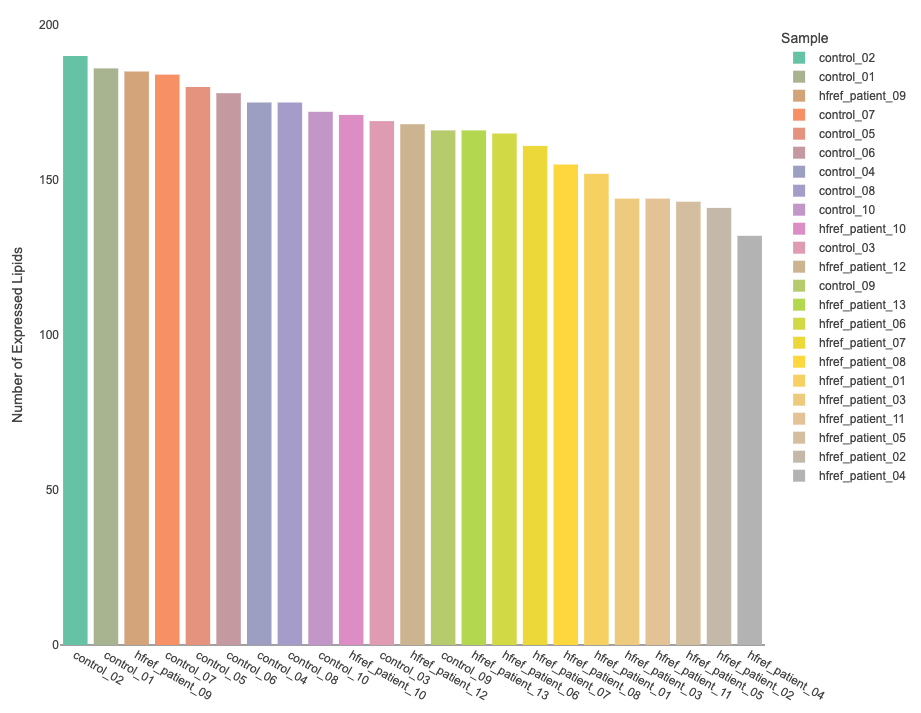
\includegraphics{./image/exp_profilling_1.png}

\begin{Shaded}
\begin{Highlighting}[]
\CommentTok{# view result: histogram (total amount of lipid)}
\NormalTok{profiling_result}\OperatorTok{$}\NormalTok{i.p.amount      }
\end{Highlighting}
\end{Shaded}

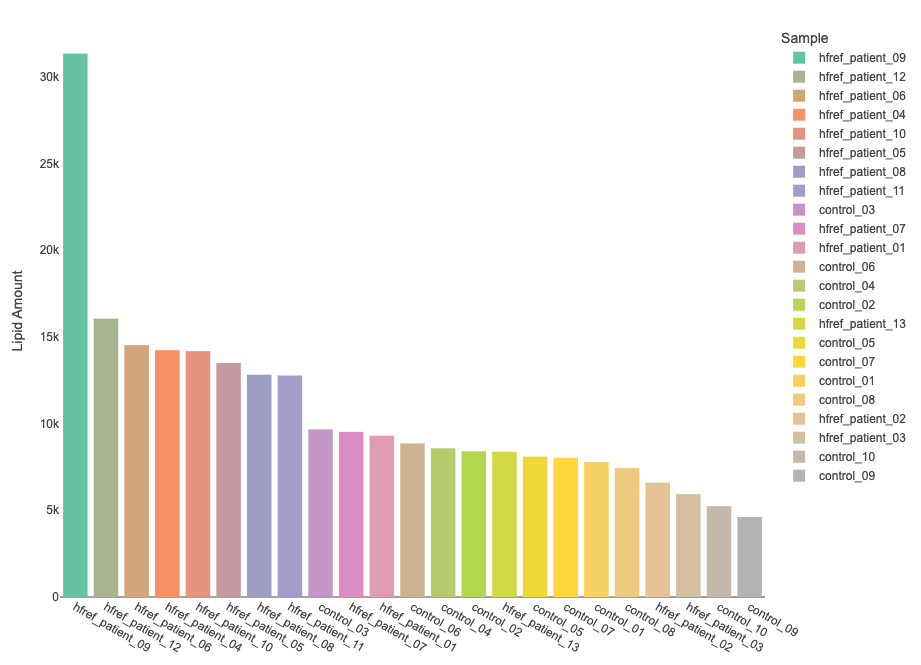
\includegraphics{./image/exp_profilling_2.png}

\begin{Shaded}
\begin{Highlighting}[]
\CommentTok{# view result: density plot of expression distribution}
\NormalTok{profiling_result}\OperatorTok{$}\NormalTok{p.hist.value}
\end{Highlighting}
\end{Shaded}

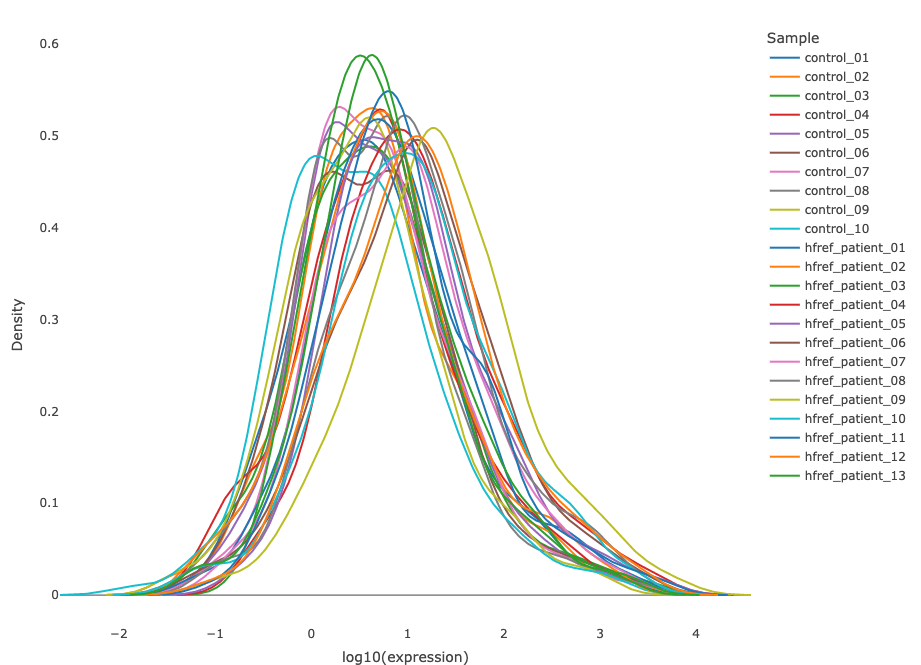
\includegraphics{./image/exp_profilling_3.png}

\hypertarget{DimensionReduce}{%
\section{Dimensionality reduction}\label{DimensionReduce}}

Dimensionality reduction is commonly used when dealing with large numbers of observations and/or large numbers of variables in lipids analysis. It transforms data from a high-dimensional space into a low-dimensional space so that it retains vital properties of the original data and is close to its intrinsic dimension.

Here we provide 3 dimensionality reduction methods and 4 clustering methods. As for the number of groups shown on the PCA, t-SNE, and UMAP plot, it can be defined by users (default: 2 groups).

\begin{enumerate}
\def\labelenumi{\arabic{enumi}.}
\tightlist
\item
  \textbf{Dimensionality reduction methods}: PCA, t-SNE, UMAP.
\item
  \textbf{Clustering methods}: K-means, partitioning around medoids (PAM), Hierarchical clustering, and DBSCAN
\end{enumerate}

\hypertarget{PCA}{%
\subsection{PCA}\label{PCA}}

PCA (Principal component analysis) is an unsupervised linear dimensionality reduction and data visualization technique for high dimensional data, which tries to preserve the global structure of the data. Scaling (by default) indicates that the variables should be scaled to have unit variance before the analysis takes place, which removes the bias towards high variances. In general, scaling (standardization) is advisable for data transformation when the variables in the original dataset have been measured on a significantly different scale. As for the centering options (by default), we offer the option of mean-centering, subtracting the mean of each variable from the values, making the mean of each variable equal to zero. It can help users to avoid the interference of misleading information given by the overall mean.

\begin{Shaded}
\begin{Highlighting}[]
\CommentTok{# data processing of exp_data}
\NormalTok{exp_transform_table <-}\StringTok{ }\KeywordTok{data_process}\NormalTok{(exp_data, }\DataTypeTok{exclude_var_missing=}\OtherTok{TRUE}\NormalTok{,}
                                    \DataTypeTok{missing_pct_limit=}\DecValTok{50}\NormalTok{, }
                                    \DataTypeTok{replace_zero=}\OtherTok{TRUE}\NormalTok{, }\DataTypeTok{zero2what=}\StringTok{'min'}\NormalTok{, }
                                    \DataTypeTok{xmin=}\FloatTok{0.5}\NormalTok{, }\DataTypeTok{replace_NA=}\OtherTok{TRUE}\NormalTok{,}
                                    \DataTypeTok{NA2what=}\StringTok{'min'}\NormalTok{, }\DataTypeTok{ymin=}\FloatTok{0.5}\NormalTok{, }
                                    \DataTypeTok{pct_transform=}\OtherTok{TRUE}\NormalTok{,}
                                    \DataTypeTok{data_transform=}\OtherTok{TRUE}\NormalTok{, }\DataTypeTok{trans_type=}\StringTok{'log'}\NormalTok{,}
                                    \DataTypeTok{centering=}\OtherTok{FALSE}\NormalTok{, }\DataTypeTok{scaling=}\OtherTok{FALSE}\NormalTok{)}
\CommentTok{# conduct PCA}
\NormalTok{PCA_result <-}\StringTok{ }\KeywordTok{PCA}\NormalTok{(exp_transform_table,}
                  \DataTypeTok{group_info =} \OtherTok{NULL}\NormalTok{, }\DataTypeTok{sig_feature =} \OtherTok{NULL}\NormalTok{,}
                  \DataTypeTok{scaling=}\OtherTok{TRUE}\NormalTok{, }\DataTypeTok{centering=}\OtherTok{TRUE}\NormalTok{, }\DataTypeTok{cluster_method=}\StringTok{'kmeans'}\NormalTok{,}
                  \DataTypeTok{group_num=}\DecValTok{2}\NormalTok{, }\DataTypeTok{var1 =} \OtherTok{NULL}\NormalTok{, }\DataTypeTok{var2 =} \OtherTok{NULL}\NormalTok{,}
                  \DataTypeTok{insert_ref_group=}\OtherTok{NULL}\NormalTok{, }\DataTypeTok{ref_group=}\OtherTok{NULL}\NormalTok{,}
                  \DataTypeTok{n_PC=}\KeywordTok{c}\NormalTok{(}\DecValTok{1}\NormalTok{,}\DecValTok{2}\NormalTok{), }\DataTypeTok{top_n_feature=}\DecValTok{10}\NormalTok{)}

\CommentTok{# view result: PCA prcomp}
\KeywordTok{head}\NormalTok{(PCA_result[[}\DecValTok{1}\NormalTok{]], }\DecValTok{1}\NormalTok{)}
\CommentTok{## $sdev}
\CommentTok{##  [1] 6.641716e+00 5.272274e+00 4.247168e+00 3.711370e+00 3.058461e+00}
\CommentTok{##  [6] 2.732843e+00 2.623854e+00 2.476808e+00 2.307884e+00 2.086144e+00}
\CommentTok{## [11] 1.981612e+00 1.923971e+00 1.848639e+00 1.791394e+00 1.756612e+00}
\CommentTok{## [16] 1.722894e+00 1.518288e+00 1.451361e+00 1.379832e+00 1.304074e+00}
\CommentTok{## [21] 1.181540e+00 1.018145e+00 4.242814e-15}
\end{Highlighting}
\end{Shaded}

\begin{Shaded}
\begin{Highlighting}[]
\CommentTok{# view result: PCA plot}
\NormalTok{PCA_result[[}\DecValTok{4}\NormalTok{]]}
\end{Highlighting}
\end{Shaded}

\textbackslash end\{kframe\}

\begin{figure}

{\centering 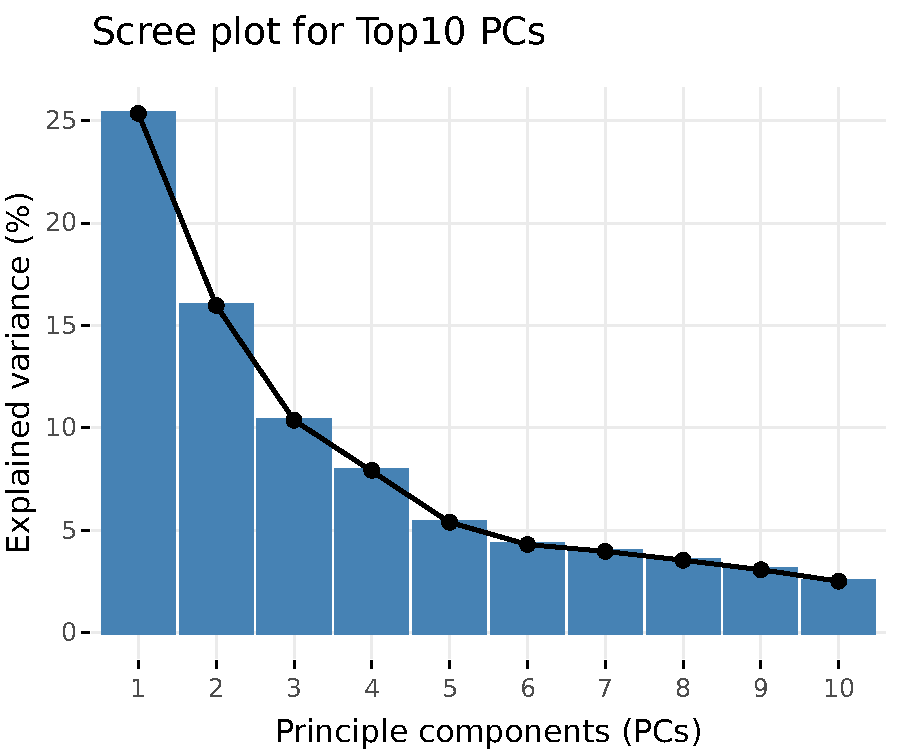
\includegraphics{Profiling_files/figure-latex/unnamed-chunk-7-1}

}

\caption{PCA plot}\label{fig:unnamed-chunk-7}
\end{figure}

\textbackslash begin\{kframe\}
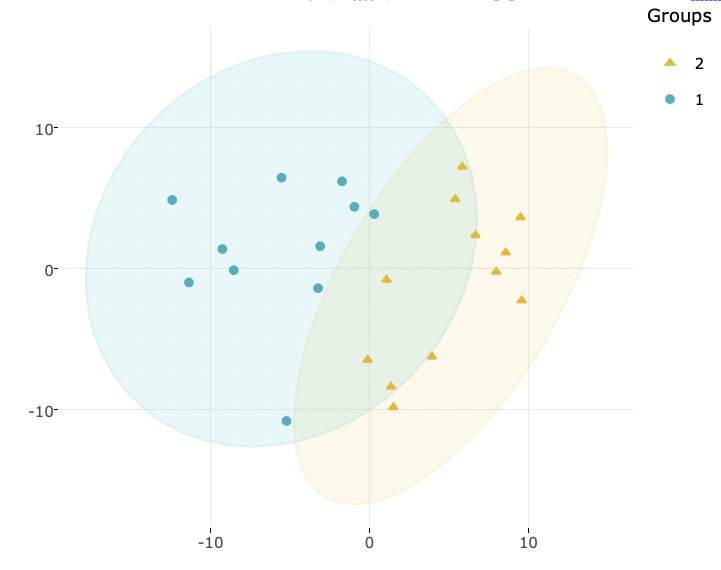
\includegraphics{./image/pca_biplot.png}
Accompanying with the PCA plot, we offer scree plot criterion, which is a common method for determining the number of PCs to be retained. The ``elbow'' of the graph indicates all components to the left of this point can explain most variability of the samples.

\begin{Shaded}
\begin{Highlighting}[]
\CommentTok{# view result: scree plot of top 10 principle components}
\NormalTok{PCA_result[[}\DecValTok{5}\NormalTok{]] }
\end{Highlighting}
\end{Shaded}

\textbackslash end\{kframe\}

\begin{figure}

{\centering 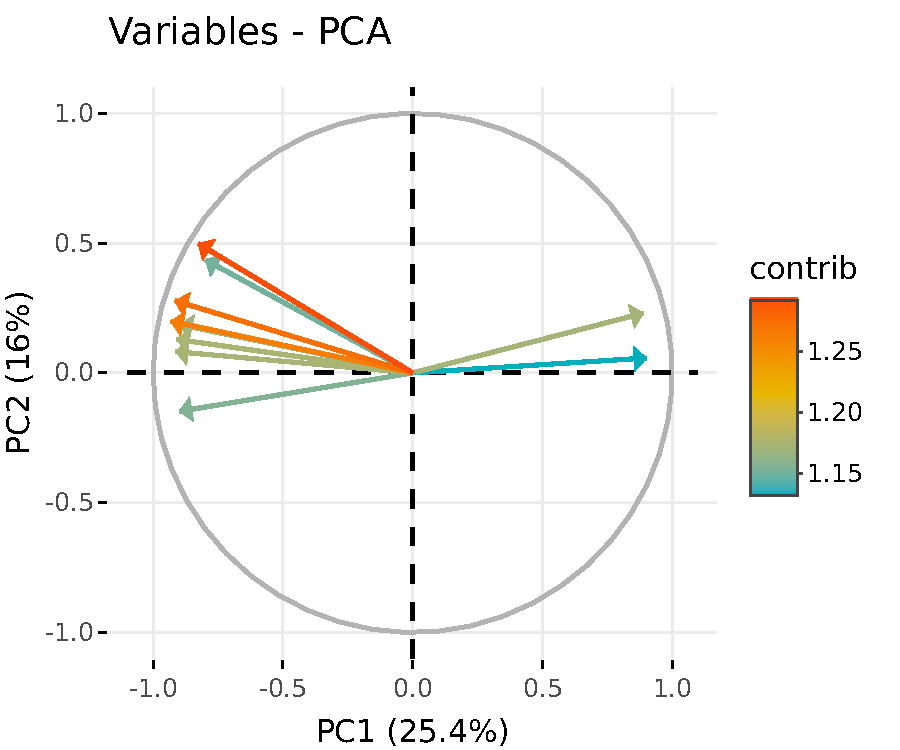
\includegraphics{Profiling_files/figure-latex/unnamed-chunk-8-1}

}

\caption{Scree plot}\label{fig:unnamed-chunk-8}
\end{figure}

\textbackslash begin\{kframe\}
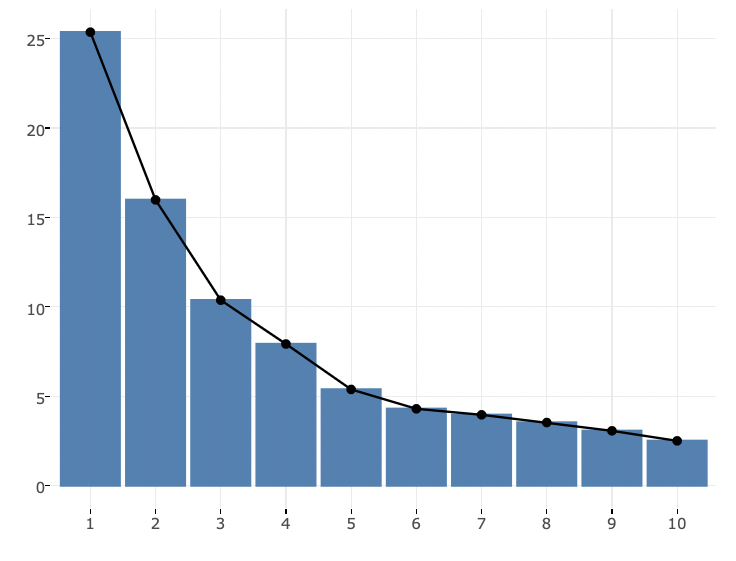
\includegraphics{./image/pca_screeplot.png}
Next, the two data frames related to PCA show the contribution to each principal component in each sample and the contribution of each feature (lipid species).

\begin{Shaded}
\begin{Highlighting}[]
\CommentTok{# view result: data frame of PCA rotated data}
\KeywordTok{head}\NormalTok{(PCA_result[[}\DecValTok{2}\NormalTok{]][,}\DecValTok{1}\OperatorTok{:}\DecValTok{5}\NormalTok{], }\DecValTok{5}\NormalTok{)}
\end{Highlighting}
\end{Shaded}


  \providecommand{\huxb}[2]{\arrayrulecolor[RGB]{#1}\global\arrayrulewidth=#2pt}
  \providecommand{\huxvb}[2]{\color[RGB]{#1}\vrule width #2pt}
  \providecommand{\huxtpad}[1]{\rule{0pt}{#1}}
  \providecommand{\huxbpad}[1]{\rule[-#1]{0pt}{#1}}

\begin{table}[ht]
\begin{centerbox}
\begin{threeparttable}
 \label{tab:unnamed-chunk-9}
\setlength{\tabcolsep}{0pt}
\begin{tabular}{l l l l l}


\hhline{>{\huxb{0, 0, 0}{0.4}}->{\huxb{0, 0, 0}{0.4}}->{\huxb{0, 0, 0}{0.4}}->{\huxb{0, 0, 0}{0.4}}->{\huxb{0, 0, 0}{0.4}}-}
\arrayrulecolor{black}

\multicolumn{1}{!{\huxvb{0, 0, 0}{0.4}}l!{\huxvb{0, 0, 0}{0}}}{\huxtpad{6pt + 1em}\raggedright \hspace{6pt} \textbf{sample\_name} \hspace{6pt}\huxbpad{6pt}} &
\multicolumn{1}{r!{\huxvb{0, 0, 0}{0}}}{\huxtpad{6pt + 1em}\raggedleft \hspace{6pt} \textbf{group} \hspace{6pt}\huxbpad{6pt}} &
\multicolumn{1}{r!{\huxvb{0, 0, 0}{0}}}{\huxtpad{6pt + 1em}\raggedleft \hspace{6pt} \textbf{PC1} \hspace{6pt}\huxbpad{6pt}} &
\multicolumn{1}{r!{\huxvb{0, 0, 0}{0}}}{\huxtpad{6pt + 1em}\raggedleft \hspace{6pt} \textbf{PC2} \hspace{6pt}\huxbpad{6pt}} &
\multicolumn{1}{r!{\huxvb{0, 0, 0}{0.4}}}{\huxtpad{6pt + 1em}\raggedleft \hspace{6pt} \textbf{PC3} \hspace{6pt}\huxbpad{6pt}} \tabularnewline[-0.5pt]


\hhline{>{\huxb{0, 0, 0}{0.4}}->{\huxb{0, 0, 0}{0.4}}->{\huxb{0, 0, 0}{0.4}}->{\huxb{0, 0, 0}{0.4}}->{\huxb{0, 0, 0}{0.4}}-}
\arrayrulecolor{black}

\multicolumn{1}{!{\huxvb{0, 0, 0}{0.4}}l!{\huxvb{0, 0, 0}{0}}}{\cellcolor[RGB]{242, 242, 242}\huxtpad{6pt + 1em}\raggedright \hspace{6pt} control\_01 \hspace{6pt}\huxbpad{6pt}} &
\multicolumn{1}{r!{\huxvb{0, 0, 0}{0}}}{\cellcolor[RGB]{242, 242, 242}\huxtpad{6pt + 1em}\raggedleft \hspace{6pt} 2 \hspace{6pt}\huxbpad{6pt}} &
\multicolumn{1}{r!{\huxvb{0, 0, 0}{0}}}{\cellcolor[RGB]{242, 242, 242}\huxtpad{6pt + 1em}\raggedleft \hspace{6pt} -1.74\hphantom{0} \hspace{6pt}\huxbpad{6pt}} &
\multicolumn{1}{r!{\huxvb{0, 0, 0}{0}}}{\cellcolor[RGB]{242, 242, 242}\huxtpad{6pt + 1em}\raggedleft \hspace{6pt} 6.17\hphantom{0} \hspace{6pt}\huxbpad{6pt}} &
\multicolumn{1}{r!{\huxvb{0, 0, 0}{0.4}}}{\cellcolor[RGB]{242, 242, 242}\huxtpad{6pt + 1em}\raggedleft \hspace{6pt} 2.88\hphantom{0} \hspace{6pt}\huxbpad{6pt}} \tabularnewline[-0.5pt]


\hhline{>{\huxb{0, 0, 0}{0.4}}|>{\huxb{0, 0, 0}{0.4}}|}
\arrayrulecolor{black}

\multicolumn{1}{!{\huxvb{0, 0, 0}{0.4}}l!{\huxvb{0, 0, 0}{0}}}{\huxtpad{6pt + 1em}\raggedright \hspace{6pt} control\_02 \hspace{6pt}\huxbpad{6pt}} &
\multicolumn{1}{r!{\huxvb{0, 0, 0}{0}}}{\huxtpad{6pt + 1em}\raggedleft \hspace{6pt} 2 \hspace{6pt}\huxbpad{6pt}} &
\multicolumn{1}{r!{\huxvb{0, 0, 0}{0}}}{\huxtpad{6pt + 1em}\raggedleft \hspace{6pt} -0.957 \hspace{6pt}\huxbpad{6pt}} &
\multicolumn{1}{r!{\huxvb{0, 0, 0}{0}}}{\huxtpad{6pt + 1em}\raggedleft \hspace{6pt} 4.36\hphantom{0} \hspace{6pt}\huxbpad{6pt}} &
\multicolumn{1}{r!{\huxvb{0, 0, 0}{0.4}}}{\huxtpad{6pt + 1em}\raggedleft \hspace{6pt} 0.695 \hspace{6pt}\huxbpad{6pt}} \tabularnewline[-0.5pt]


\hhline{>{\huxb{0, 0, 0}{0.4}}|>{\huxb{0, 0, 0}{0.4}}|}
\arrayrulecolor{black}

\multicolumn{1}{!{\huxvb{0, 0, 0}{0.4}}l!{\huxvb{0, 0, 0}{0}}}{\cellcolor[RGB]{242, 242, 242}\huxtpad{6pt + 1em}\raggedright \hspace{6pt} control\_03 \hspace{6pt}\huxbpad{6pt}} &
\multicolumn{1}{r!{\huxvb{0, 0, 0}{0}}}{\cellcolor[RGB]{242, 242, 242}\huxtpad{6pt + 1em}\raggedleft \hspace{6pt} 1 \hspace{6pt}\huxbpad{6pt}} &
\multicolumn{1}{r!{\huxvb{0, 0, 0}{0}}}{\cellcolor[RGB]{242, 242, 242}\huxtpad{6pt + 1em}\raggedleft \hspace{6pt} 7.96\hphantom{0} \hspace{6pt}\huxbpad{6pt}} &
\multicolumn{1}{r!{\huxvb{0, 0, 0}{0}}}{\cellcolor[RGB]{242, 242, 242}\huxtpad{6pt + 1em}\raggedleft \hspace{6pt} -0.249 \hspace{6pt}\huxbpad{6pt}} &
\multicolumn{1}{r!{\huxvb{0, 0, 0}{0.4}}}{\cellcolor[RGB]{242, 242, 242}\huxtpad{6pt + 1em}\raggedleft \hspace{6pt} 4.23\hphantom{0} \hspace{6pt}\huxbpad{6pt}} \tabularnewline[-0.5pt]


\hhline{>{\huxb{0, 0, 0}{0.4}}|>{\huxb{0, 0, 0}{0.4}}|}
\arrayrulecolor{black}

\multicolumn{1}{!{\huxvb{0, 0, 0}{0.4}}l!{\huxvb{0, 0, 0}{0}}}{\huxtpad{6pt + 1em}\raggedright \hspace{6pt} control\_04 \hspace{6pt}\huxbpad{6pt}} &
\multicolumn{1}{r!{\huxvb{0, 0, 0}{0}}}{\huxtpad{6pt + 1em}\raggedleft \hspace{6pt} 2 \hspace{6pt}\huxbpad{6pt}} &
\multicolumn{1}{r!{\huxvb{0, 0, 0}{0}}}{\huxtpad{6pt + 1em}\raggedleft \hspace{6pt} -3.11\hphantom{0} \hspace{6pt}\huxbpad{6pt}} &
\multicolumn{1}{r!{\huxvb{0, 0, 0}{0}}}{\huxtpad{6pt + 1em}\raggedleft \hspace{6pt} 1.57\hphantom{0} \hspace{6pt}\huxbpad{6pt}} &
\multicolumn{1}{r!{\huxvb{0, 0, 0}{0.4}}}{\huxtpad{6pt + 1em}\raggedleft \hspace{6pt} 6.71\hphantom{0} \hspace{6pt}\huxbpad{6pt}} \tabularnewline[-0.5pt]


\hhline{>{\huxb{0, 0, 0}{0.4}}|>{\huxb{0, 0, 0}{0.4}}|}
\arrayrulecolor{black}

\multicolumn{1}{!{\huxvb{0, 0, 0}{0.4}}l!{\huxvb{0, 0, 0}{0}}}{\cellcolor[RGB]{242, 242, 242}\huxtpad{6pt + 1em}\raggedright \hspace{6pt} control\_05 \hspace{6pt}\huxbpad{6pt}} &
\multicolumn{1}{r!{\huxvb{0, 0, 0}{0}}}{\cellcolor[RGB]{242, 242, 242}\huxtpad{6pt + 1em}\raggedleft \hspace{6pt} 1 \hspace{6pt}\huxbpad{6pt}} &
\multicolumn{1}{r!{\huxvb{0, 0, 0}{0}}}{\cellcolor[RGB]{242, 242, 242}\huxtpad{6pt + 1em}\raggedleft \hspace{6pt} 5.83\hphantom{0} \hspace{6pt}\huxbpad{6pt}} &
\multicolumn{1}{r!{\huxvb{0, 0, 0}{0}}}{\cellcolor[RGB]{242, 242, 242}\huxtpad{6pt + 1em}\raggedleft \hspace{6pt} 7.2\hphantom{0}\hphantom{0} \hspace{6pt}\huxbpad{6pt}} &
\multicolumn{1}{r!{\huxvb{0, 0, 0}{0.4}}}{\cellcolor[RGB]{242, 242, 242}\huxtpad{6pt + 1em}\raggedleft \hspace{6pt} 0.154 \hspace{6pt}\huxbpad{6pt}} \tabularnewline[-0.5pt]


\hhline{>{\huxb{0, 0, 0}{0.4}}->{\huxb{0, 0, 0}{0.4}}->{\huxb{0, 0, 0}{0.4}}->{\huxb{0, 0, 0}{0.4}}->{\huxb{0, 0, 0}{0.4}}-}
\arrayrulecolor{black}
\end{tabular}
\end{threeparttable}\par\end{centerbox}

\end{table}

# view result: data frame of PCA contribution table
head(PCA_result[[3]][,1:5], 5)


  \providecommand{\huxb}[2]{\arrayrulecolor[RGB]{#1}\global\arrayrulewidth=#2pt}
  \providecommand{\huxvb}[2]{\color[RGB]{#1}\vrule width #2pt}
  \providecommand{\huxtpad}[1]{\rule{0pt}{#1}}
  \providecommand{\huxbpad}[1]{\rule[-#1]{0pt}{#1}}

\begin{table}[ht]
\begin{centerbox}
\begin{threeparttable}
 \label{tab:unnamed-chunk-9}
\setlength{\tabcolsep}{0pt}
\begin{tabular}{l l l l l}


\hhline{>{\huxb{0, 0, 0}{0.4}}->{\huxb{0, 0, 0}{0.4}}->{\huxb{0, 0, 0}{0.4}}->{\huxb{0, 0, 0}{0.4}}->{\huxb{0, 0, 0}{0.4}}-}
\arrayrulecolor{black}

\multicolumn{1}{!{\huxvb{0, 0, 0}{0.4}}l!{\huxvb{0, 0, 0}{0}}}{\huxtpad{6pt + 1em}\raggedright \hspace{6pt} \textbf{feature} \hspace{6pt}\huxbpad{6pt}} &
\multicolumn{1}{r!{\huxvb{0, 0, 0}{0}}}{\huxtpad{6pt + 1em}\raggedleft \hspace{6pt} \textbf{PC1} \hspace{6pt}\huxbpad{6pt}} &
\multicolumn{1}{r!{\huxvb{0, 0, 0}{0}}}{\huxtpad{6pt + 1em}\raggedleft \hspace{6pt} \textbf{PC2} \hspace{6pt}\huxbpad{6pt}} &
\multicolumn{1}{r!{\huxvb{0, 0, 0}{0}}}{\huxtpad{6pt + 1em}\raggedleft \hspace{6pt} \textbf{PC3} \hspace{6pt}\huxbpad{6pt}} &
\multicolumn{1}{r!{\huxvb{0, 0, 0}{0.4}}}{\huxtpad{6pt + 1em}\raggedleft \hspace{6pt} \textbf{PC4} \hspace{6pt}\huxbpad{6pt}} \tabularnewline[-0.5pt]


\hhline{>{\huxb{0, 0, 0}{0.4}}->{\huxb{0, 0, 0}{0.4}}->{\huxb{0, 0, 0}{0.4}}->{\huxb{0, 0, 0}{0.4}}->{\huxb{0, 0, 0}{0.4}}-}
\arrayrulecolor{black}

\multicolumn{1}{!{\huxvb{0, 0, 0}{0.4}}l!{\huxvb{0, 0, 0}{0}}}{\cellcolor[RGB]{242, 242, 242}\huxtpad{6pt + 1em}\raggedright \hspace{6pt} Cer 38:1;2 \hspace{6pt}\huxbpad{6pt}} &
\multicolumn{1}{r!{\huxvb{0, 0, 0}{0}}}{\cellcolor[RGB]{242, 242, 242}\huxtpad{6pt + 1em}\raggedleft \hspace{6pt} 0.000124 \hspace{6pt}\huxbpad{6pt}} &
\multicolumn{1}{r!{\huxvb{0, 0, 0}{0}}}{\cellcolor[RGB]{242, 242, 242}\huxtpad{6pt + 1em}\raggedleft \hspace{6pt} 0.537\hphantom{0} \hspace{6pt}\huxbpad{6pt}} &
\multicolumn{1}{r!{\huxvb{0, 0, 0}{0}}}{\cellcolor[RGB]{242, 242, 242}\huxtpad{6pt + 1em}\raggedleft \hspace{6pt} 0.762\hphantom{0}\hphantom{0} \hspace{6pt}\huxbpad{6pt}} &
\multicolumn{1}{r!{\huxvb{0, 0, 0}{0.4}}}{\cellcolor[RGB]{242, 242, 242}\huxtpad{6pt + 1em}\raggedleft \hspace{6pt} 0.52\hphantom{0} \hspace{6pt}\huxbpad{6pt}} \tabularnewline[-0.5pt]


\hhline{>{\huxb{0, 0, 0}{0.4}}|>{\huxb{0, 0, 0}{0.4}}|}
\arrayrulecolor{black}

\multicolumn{1}{!{\huxvb{0, 0, 0}{0.4}}l!{\huxvb{0, 0, 0}{0}}}{\huxtpad{6pt + 1em}\raggedright \hspace{6pt} Cer 40:1;2 \hspace{6pt}\huxbpad{6pt}} &
\multicolumn{1}{r!{\huxvb{0, 0, 0}{0}}}{\huxtpad{6pt + 1em}\raggedleft \hspace{6pt} 0.0501\hphantom{0}\hphantom{0} \hspace{6pt}\huxbpad{6pt}} &
\multicolumn{1}{r!{\huxvb{0, 0, 0}{0}}}{\huxtpad{6pt + 1em}\raggedleft \hspace{6pt} 0.763\hphantom{0} \hspace{6pt}\huxbpad{6pt}} &
\multicolumn{1}{r!{\huxvb{0, 0, 0}{0}}}{\huxtpad{6pt + 1em}\raggedleft \hspace{6pt} 0.00969 \hspace{6pt}\huxbpad{6pt}} &
\multicolumn{1}{r!{\huxvb{0, 0, 0}{0.4}}}{\huxtpad{6pt + 1em}\raggedleft \hspace{6pt} 1.41\hphantom{0} \hspace{6pt}\huxbpad{6pt}} \tabularnewline[-0.5pt]


\hhline{>{\huxb{0, 0, 0}{0.4}}|>{\huxb{0, 0, 0}{0.4}}|}
\arrayrulecolor{black}

\multicolumn{1}{!{\huxvb{0, 0, 0}{0.4}}l!{\huxvb{0, 0, 0}{0}}}{\cellcolor[RGB]{242, 242, 242}\huxtpad{6pt + 1em}\raggedright \hspace{6pt} Cer 40:2;2 \hspace{6pt}\huxbpad{6pt}} &
\multicolumn{1}{r!{\huxvb{0, 0, 0}{0}}}{\cellcolor[RGB]{242, 242, 242}\huxtpad{6pt + 1em}\raggedleft \hspace{6pt} 0.0154\hphantom{0}\hphantom{0} \hspace{6pt}\huxbpad{6pt}} &
\multicolumn{1}{r!{\huxvb{0, 0, 0}{0}}}{\cellcolor[RGB]{242, 242, 242}\huxtpad{6pt + 1em}\raggedleft \hspace{6pt} 0.355\hphantom{0} \hspace{6pt}\huxbpad{6pt}} &
\multicolumn{1}{r!{\huxvb{0, 0, 0}{0}}}{\cellcolor[RGB]{242, 242, 242}\huxtpad{6pt + 1em}\raggedleft \hspace{6pt} 0.0362\hphantom{0} \hspace{6pt}\huxbpad{6pt}} &
\multicolumn{1}{r!{\huxvb{0, 0, 0}{0.4}}}{\cellcolor[RGB]{242, 242, 242}\huxtpad{6pt + 1em}\raggedleft \hspace{6pt} 3.21\hphantom{0} \hspace{6pt}\huxbpad{6pt}} \tabularnewline[-0.5pt]


\hhline{>{\huxb{0, 0, 0}{0.4}}|>{\huxb{0, 0, 0}{0.4}}|}
\arrayrulecolor{black}

\multicolumn{1}{!{\huxvb{0, 0, 0}{0.4}}l!{\huxvb{0, 0, 0}{0}}}{\huxtpad{6pt + 1em}\raggedright \hspace{6pt} Cer 42:1;2 \hspace{6pt}\huxbpad{6pt}} &
\multicolumn{1}{r!{\huxvb{0, 0, 0}{0}}}{\huxtpad{6pt + 1em}\raggedleft \hspace{6pt} 0.0175\hphantom{0}\hphantom{0} \hspace{6pt}\huxbpad{6pt}} &
\multicolumn{1}{r!{\huxvb{0, 0, 0}{0}}}{\huxtpad{6pt + 1em}\raggedleft \hspace{6pt} 0.617\hphantom{0} \hspace{6pt}\huxbpad{6pt}} &
\multicolumn{1}{r!{\huxvb{0, 0, 0}{0}}}{\huxtpad{6pt + 1em}\raggedleft \hspace{6pt} 0.634\hphantom{0}\hphantom{0} \hspace{6pt}\huxbpad{6pt}} &
\multicolumn{1}{r!{\huxvb{0, 0, 0}{0.4}}}{\huxtpad{6pt + 1em}\raggedleft \hspace{6pt} 1.8\hphantom{0}\hphantom{0} \hspace{6pt}\huxbpad{6pt}} \tabularnewline[-0.5pt]


\hhline{>{\huxb{0, 0, 0}{0.4}}|>{\huxb{0, 0, 0}{0.4}}|}
\arrayrulecolor{black}

\multicolumn{1}{!{\huxvb{0, 0, 0}{0.4}}l!{\huxvb{0, 0, 0}{0}}}{\cellcolor[RGB]{242, 242, 242}\huxtpad{6pt + 1em}\raggedright \hspace{6pt} Cer 42:2;2 \hspace{6pt}\huxbpad{6pt}} &
\multicolumn{1}{r!{\huxvb{0, 0, 0}{0}}}{\cellcolor[RGB]{242, 242, 242}\huxtpad{6pt + 1em}\raggedleft \hspace{6pt} 0.000479 \hspace{6pt}\huxbpad{6pt}} &
\multicolumn{1}{r!{\huxvb{0, 0, 0}{0}}}{\cellcolor[RGB]{242, 242, 242}\huxtpad{6pt + 1em}\raggedleft \hspace{6pt} 0.0624 \hspace{6pt}\huxbpad{6pt}} &
\multicolumn{1}{r!{\huxvb{0, 0, 0}{0}}}{\cellcolor[RGB]{242, 242, 242}\huxtpad{6pt + 1em}\raggedleft \hspace{6pt} 0.00208 \hspace{6pt}\huxbpad{6pt}} &
\multicolumn{1}{r!{\huxvb{0, 0, 0}{0.4}}}{\cellcolor[RGB]{242, 242, 242}\huxtpad{6pt + 1em}\raggedleft \hspace{6pt} 0.621 \hspace{6pt}\huxbpad{6pt}} \tabularnewline[-0.5pt]


\hhline{>{\huxb{0, 0, 0}{0.4}}->{\huxb{0, 0, 0}{0.4}}->{\huxb{0, 0, 0}{0.4}}->{\huxb{0, 0, 0}{0.4}}->{\huxb{0, 0, 0}{0.4}}-}
\arrayrulecolor{black}
\end{tabular}
\end{threeparttable}\par\end{centerbox}

\end{table}


Following is the correlation circle plot that reveals the relationships between all variables.

\begin{Shaded}
\begin{Highlighting}[]
\CommentTok{# view result: correlation circle plot of PCA variables}
\NormalTok{PCA_result[[}\DecValTok{7}\NormalTok{]]}
\end{Highlighting}
\end{Shaded}

\textbackslash end\{kframe\}

\begin{figure}

{\centering 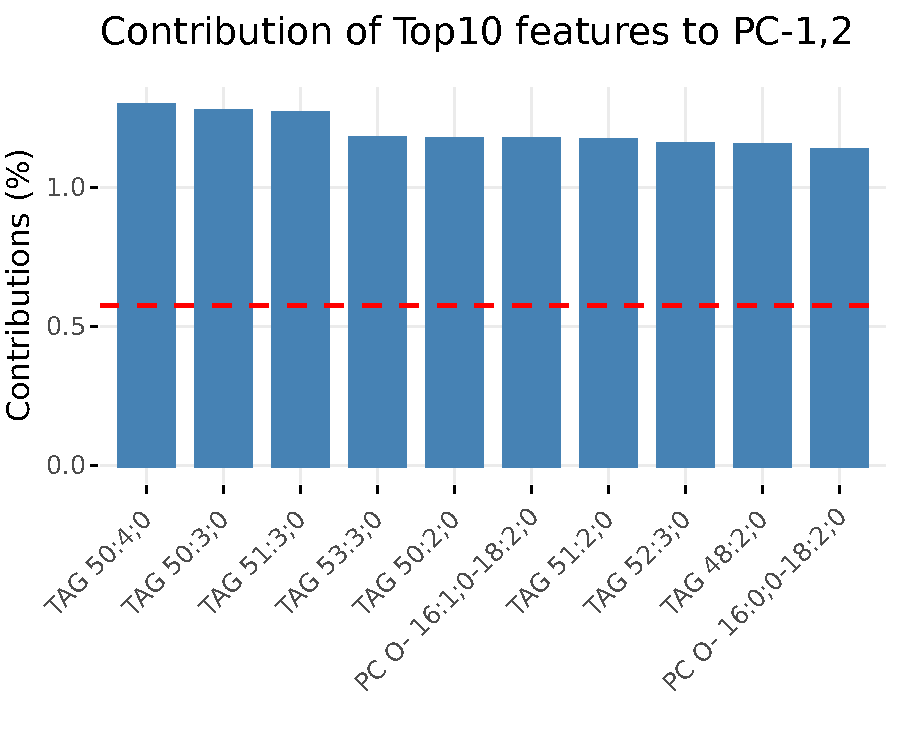
\includegraphics{Profiling_files/figure-latex/unnamed-chunk-10-1}

}

\caption{Correlation circle plot. The correlation circle plot showing the correlation between a feature (lipid species) and a principal component (PC) used as the coordinates of the variable on the PC [@abdi2010principal]. The positively correlated variables are in the same quadrants while negatively correlated variables are on the opposite sides of the plot origin. The closer a variable to the edge of the circle, the better it represents on the factor map.}\label{fig:unnamed-chunk-10}
\end{figure}

\textbackslash begin\{kframe\}
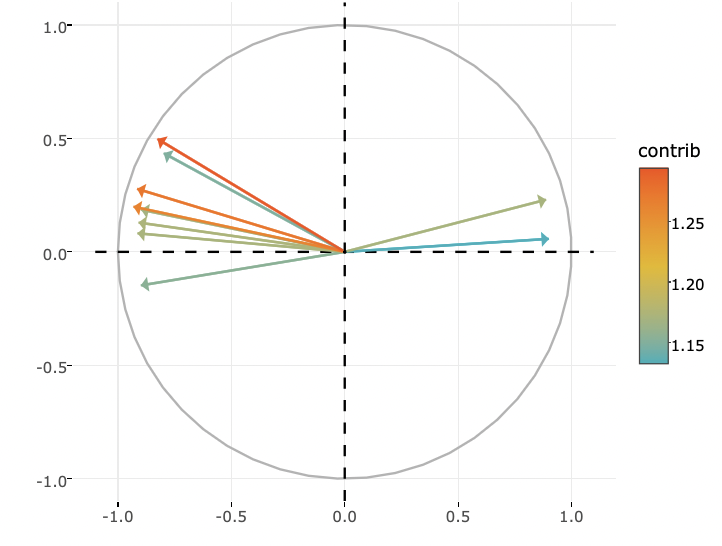
\includegraphics{./image/pca_variable.png}

Lastly, we can have a closer look at the contribution of top 10 features to a user-defined principal component (e.g., PC1, PC2, or PC1+PC2). Therefore, in the histogram, we can find out the features (lipid species) that contribute more to the user-defined principal component.

\begin{Shaded}
\begin{Highlighting}[]
\CommentTok{# view result: bar plot of contribution of top 10 features}
\NormalTok{PCA_result[[}\DecValTok{6}\NormalTok{]]  }
\end{Highlighting}
\end{Shaded}

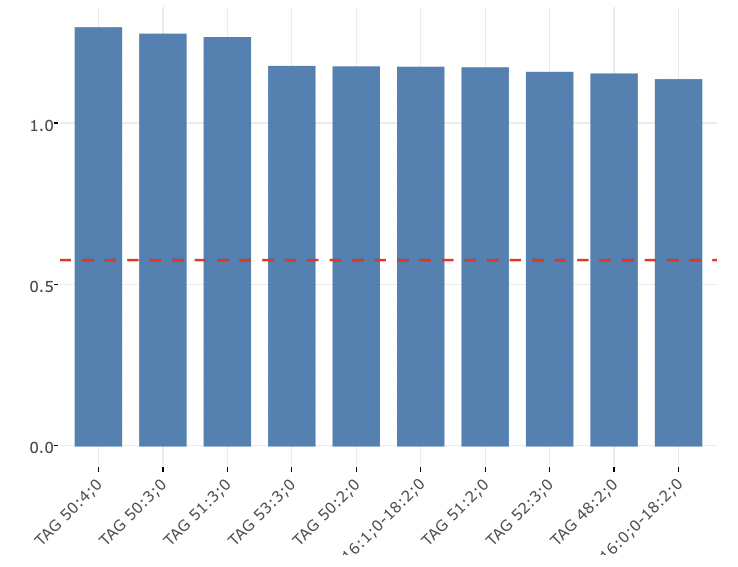
\includegraphics{./image/pca_feature_contrib.png}

\hypertarget{t-SNE}{%
\subsection{t-SNE}\label{t-SNE}}

t-SNE (t-Distributed Stochastic Neighbour Embedding) is an unsupervised non-linear dimensionality reduction technique that tries to retain the local structure(cluster) of data when visualising the high-dimensional datasets. Package \emph{\href{https://CRAN.R-project.org/package=Rtsne}{Rtsne}} is used for calculation, and PCA is applied as a pre-processing step. In t-SNE, \texttt{perplexity} and \texttt{max\_iter} are adjustable for users. The \texttt{perplexity} may be considered as a knob that sets the number of effective nearest neighbours, while \texttt{max\_iter} is the maximum number of iterations to perform. The typical perplexity range between 5 and 50, but if the t-SNE plot shows a `ball' with uniformly distributed points, you may need to lower your perplexity.\textsuperscript{1}

\begin{Shaded}
\begin{Highlighting}[]
\CommentTok{# data processing of exp_data}
\NormalTok{exp_transform_table <-}\StringTok{ }\KeywordTok{data_process}\NormalTok{(exp_data, }\DataTypeTok{exclude_var_missing=}\OtherTok{TRUE}\NormalTok{,}
                                    \DataTypeTok{missing_pct_limit=}\DecValTok{50}\NormalTok{, }
                                    \DataTypeTok{replace_zero=}\OtherTok{TRUE}\NormalTok{, }\DataTypeTok{zero2what=}\StringTok{'min'}\NormalTok{, }
                                    \DataTypeTok{xmin=}\FloatTok{0.5}\NormalTok{, }\DataTypeTok{replace_NA=}\OtherTok{TRUE}\NormalTok{,}
                                    \DataTypeTok{NA2what=}\StringTok{'min'}\NormalTok{, }\DataTypeTok{ymin=}\FloatTok{0.5}\NormalTok{, }
                                    \DataTypeTok{pct_transform=}\OtherTok{TRUE}\NormalTok{,}
                                    \DataTypeTok{data_transform=}\OtherTok{TRUE}\NormalTok{, }\DataTypeTok{trans_type=}\StringTok{'log'}\NormalTok{,}
                                    \DataTypeTok{centering=}\OtherTok{FALSE}\NormalTok{, }\DataTypeTok{scaling=}\OtherTok{FALSE}\NormalTok{)}
\CommentTok{# conduct t-SNE}
\NormalTok{tsne_result <-}\StringTok{ }\KeywordTok{tsne}\NormalTok{(exp_transform_table, }\DataTypeTok{group_info =} \OtherTok{NULL}\NormalTok{,}
                    \DataTypeTok{sig_feature =} \OtherTok{NULL}\NormalTok{, }\DataTypeTok{pca=}\OtherTok{TRUE}\NormalTok{, }\DataTypeTok{perplexity=}\DecValTok{5}\NormalTok{,}
                    \DataTypeTok{max_iter=}\DecValTok{500}\NormalTok{, }\DataTypeTok{cluster_method=}\StringTok{'kmeans'}\NormalTok{,}
                    \DataTypeTok{group_num=}\DecValTok{2}\NormalTok{, }\DataTypeTok{var1 =} \StringTok{'euclidean'}\NormalTok{, }\DataTypeTok{var2 =} \OtherTok{NULL}\NormalTok{,}
                    \DataTypeTok{insert_ref_group =} \OtherTok{NULL}\NormalTok{, }\DataTypeTok{ref_group =} \OtherTok{NULL}\NormalTok{)}
\CommentTok{## Performing PCA}
\CommentTok{## Read the 23 x 23 data matrix successfully!}
\CommentTok{## OpenMP is working. 1 threads.}
\CommentTok{## Using no_dims = 2, perplexity = 5.000000, and theta = 0.000000}
\CommentTok{## Computing input similarities...}
\CommentTok{## Symmetrizing...}
\CommentTok{## Done in 0.00 seconds!}
\CommentTok{## Learning embedding...}
\CommentTok{## Iteration 50: error is 56.209723 (50 iterations in 0.00 seconds)}
\CommentTok{## Iteration 100: error is 55.758445 (50 iterations in 0.00 seconds)}
\CommentTok{## Iteration 150: error is 52.690401 (50 iterations in 0.00 seconds)}
\CommentTok{## Iteration 200: error is 58.746613 (50 iterations in 0.00 seconds)}
\CommentTok{## Iteration 250: error is 55.783463 (50 iterations in 0.00 seconds)}
\CommentTok{## Iteration 300: error is 1.475388 (50 iterations in 0.00 seconds)}
\CommentTok{## Iteration 350: error is 1.079724 (50 iterations in 0.00 seconds)}
\CommentTok{## Iteration 400: error is 0.875064 (50 iterations in 0.00 seconds)}
\CommentTok{## Iteration 450: error is 0.634750 (50 iterations in 0.00 seconds)}
\CommentTok{## Iteration 500: error is 0.550634 (50 iterations in 0.00 seconds)}
\CommentTok{## Fitting performed in 0.00 seconds.}
\CommentTok{# view result: data frame of t-SNE data}
\KeywordTok{head}\NormalTok{(tsne_result[[}\DecValTok{1}\NormalTok{]], }\DecValTok{5}\NormalTok{)}
\end{Highlighting}
\end{Shaded}


  \providecommand{\huxb}[2]{\arrayrulecolor[RGB]{#1}\global\arrayrulewidth=#2pt}
  \providecommand{\huxvb}[2]{\color[RGB]{#1}\vrule width #2pt}
  \providecommand{\huxtpad}[1]{\rule{0pt}{#1}}
  \providecommand{\huxbpad}[1]{\rule[-#1]{0pt}{#1}}

\begin{table}[ht]
\begin{centerbox}
\begin{threeparttable}
 \label{tab:Profiling: dimensionality reduction - t-SNE}
\setlength{\tabcolsep}{0pt}
\begin{tabular}{l l l l}


\hhline{>{\huxb{0, 0, 0}{0.4}}->{\huxb{0, 0, 0}{0.4}}->{\huxb{0, 0, 0}{0.4}}->{\huxb{0, 0, 0}{0.4}}-}
\arrayrulecolor{black}

\multicolumn{1}{!{\huxvb{0, 0, 0}{0.4}}l!{\huxvb{0, 0, 0}{0}}}{\huxtpad{6pt + 1em}\raggedright \hspace{6pt} \textbf{sample\_name} \hspace{6pt}\huxbpad{6pt}} &
\multicolumn{1}{l!{\huxvb{0, 0, 0}{0}}}{\huxtpad{6pt + 1em}\raggedright \hspace{6pt} \textbf{group} \hspace{6pt}\huxbpad{6pt}} &
\multicolumn{1}{r!{\huxvb{0, 0, 0}{0}}}{\huxtpad{6pt + 1em}\raggedleft \hspace{6pt} \textbf{tsne1} \hspace{6pt}\huxbpad{6pt}} &
\multicolumn{1}{r!{\huxvb{0, 0, 0}{0.4}}}{\huxtpad{6pt + 1em}\raggedleft \hspace{6pt} \textbf{tsne2} \hspace{6pt}\huxbpad{6pt}} \tabularnewline[-0.5pt]


\hhline{>{\huxb{0, 0, 0}{0.4}}->{\huxb{0, 0, 0}{0.4}}->{\huxb{0, 0, 0}{0.4}}->{\huxb{0, 0, 0}{0.4}}-}
\arrayrulecolor{black}

\multicolumn{1}{!{\huxvb{0, 0, 0}{0.4}}l!{\huxvb{0, 0, 0}{0}}}{\cellcolor[RGB]{242, 242, 242}\huxtpad{6pt + 1em}\raggedright \hspace{6pt} control\_01 \hspace{6pt}\huxbpad{6pt}} &
\multicolumn{1}{l!{\huxvb{0, 0, 0}{0}}}{\cellcolor[RGB]{242, 242, 242}\huxtpad{6pt + 1em}\raggedright \hspace{6pt} 1 \hspace{6pt}\huxbpad{6pt}} &
\multicolumn{1}{r!{\huxvb{0, 0, 0}{0}}}{\cellcolor[RGB]{242, 242, 242}\huxtpad{6pt + 1em}\raggedleft \hspace{6pt} -22.1\hphantom{0}\hphantom{0} \hspace{6pt}\huxbpad{6pt}} &
\multicolumn{1}{r!{\huxvb{0, 0, 0}{0.4}}}{\cellcolor[RGB]{242, 242, 242}\huxtpad{6pt + 1em}\raggedleft \hspace{6pt} -48.6 \hspace{6pt}\huxbpad{6pt}} \tabularnewline[-0.5pt]


\hhline{>{\huxb{0, 0, 0}{0.4}}|>{\huxb{0, 0, 0}{0.4}}|}
\arrayrulecolor{black}

\multicolumn{1}{!{\huxvb{0, 0, 0}{0.4}}l!{\huxvb{0, 0, 0}{0}}}{\huxtpad{6pt + 1em}\raggedright \hspace{6pt} control\_02 \hspace{6pt}\huxbpad{6pt}} &
\multicolumn{1}{l!{\huxvb{0, 0, 0}{0}}}{\huxtpad{6pt + 1em}\raggedright \hspace{6pt} 1 \hspace{6pt}\huxbpad{6pt}} &
\multicolumn{1}{r!{\huxvb{0, 0, 0}{0}}}{\huxtpad{6pt + 1em}\raggedleft \hspace{6pt} 0.433 \hspace{6pt}\huxbpad{6pt}} &
\multicolumn{1}{r!{\huxvb{0, 0, 0}{0.4}}}{\huxtpad{6pt + 1em}\raggedleft \hspace{6pt} -43.2 \hspace{6pt}\huxbpad{6pt}} \tabularnewline[-0.5pt]


\hhline{>{\huxb{0, 0, 0}{0.4}}|>{\huxb{0, 0, 0}{0.4}}|}
\arrayrulecolor{black}

\multicolumn{1}{!{\huxvb{0, 0, 0}{0.4}}l!{\huxvb{0, 0, 0}{0}}}{\cellcolor[RGB]{242, 242, 242}\huxtpad{6pt + 1em}\raggedright \hspace{6pt} control\_03 \hspace{6pt}\huxbpad{6pt}} &
\multicolumn{1}{l!{\huxvb{0, 0, 0}{0}}}{\cellcolor[RGB]{242, 242, 242}\huxtpad{6pt + 1em}\raggedright \hspace{6pt} 2 \hspace{6pt}\huxbpad{6pt}} &
\multicolumn{1}{r!{\huxvb{0, 0, 0}{0}}}{\cellcolor[RGB]{242, 242, 242}\huxtpad{6pt + 1em}\raggedleft \hspace{6pt} 43.4\hphantom{0}\hphantom{0} \hspace{6pt}\huxbpad{6pt}} &
\multicolumn{1}{r!{\huxvb{0, 0, 0}{0.4}}}{\cellcolor[RGB]{242, 242, 242}\huxtpad{6pt + 1em}\raggedleft \hspace{6pt} 84.7 \hspace{6pt}\huxbpad{6pt}} \tabularnewline[-0.5pt]


\hhline{>{\huxb{0, 0, 0}{0.4}}|>{\huxb{0, 0, 0}{0.4}}|}
\arrayrulecolor{black}

\multicolumn{1}{!{\huxvb{0, 0, 0}{0.4}}l!{\huxvb{0, 0, 0}{0}}}{\huxtpad{6pt + 1em}\raggedright \hspace{6pt} control\_04 \hspace{6pt}\huxbpad{6pt}} &
\multicolumn{1}{l!{\huxvb{0, 0, 0}{0}}}{\huxtpad{6pt + 1em}\raggedright \hspace{6pt} 1 \hspace{6pt}\huxbpad{6pt}} &
\multicolumn{1}{r!{\huxvb{0, 0, 0}{0}}}{\huxtpad{6pt + 1em}\raggedleft \hspace{6pt} -18.6\hphantom{0}\hphantom{0} \hspace{6pt}\huxbpad{6pt}} &
\multicolumn{1}{r!{\huxvb{0, 0, 0}{0.4}}}{\huxtpad{6pt + 1em}\raggedleft \hspace{6pt} -25.5 \hspace{6pt}\huxbpad{6pt}} \tabularnewline[-0.5pt]


\hhline{>{\huxb{0, 0, 0}{0.4}}|>{\huxb{0, 0, 0}{0.4}}|}
\arrayrulecolor{black}

\multicolumn{1}{!{\huxvb{0, 0, 0}{0.4}}l!{\huxvb{0, 0, 0}{0}}}{\cellcolor[RGB]{242, 242, 242}\huxtpad{6pt + 1em}\raggedright \hspace{6pt} control\_05 \hspace{6pt}\huxbpad{6pt}} &
\multicolumn{1}{l!{\huxvb{0, 0, 0}{0}}}{\cellcolor[RGB]{242, 242, 242}\huxtpad{6pt + 1em}\raggedright \hspace{6pt} 1 \hspace{6pt}\huxbpad{6pt}} &
\multicolumn{1}{r!{\huxvb{0, 0, 0}{0}}}{\cellcolor[RGB]{242, 242, 242}\huxtpad{6pt + 1em}\raggedleft \hspace{6pt} -31.2\hphantom{0}\hphantom{0} \hspace{6pt}\huxbpad{6pt}} &
\multicolumn{1}{r!{\huxvb{0, 0, 0}{0.4}}}{\cellcolor[RGB]{242, 242, 242}\huxtpad{6pt + 1em}\raggedleft \hspace{6pt} -72.3 \hspace{6pt}\huxbpad{6pt}} \tabularnewline[-0.5pt]


\hhline{>{\huxb{0, 0, 0}{0.4}}->{\huxb{0, 0, 0}{0.4}}->{\huxb{0, 0, 0}{0.4}}->{\huxb{0, 0, 0}{0.4}}-}
\arrayrulecolor{black}
\end{tabular}
\end{threeparttable}\par\end{centerbox}

\end{table}


\begin{Shaded}
\begin{Highlighting}[]
\CommentTok{# view result: t-SNE plot}
\NormalTok{tsne_result[[}\DecValTok{2}\NormalTok{]] }
\end{Highlighting}
\end{Shaded}

\begin{figure}
\centering
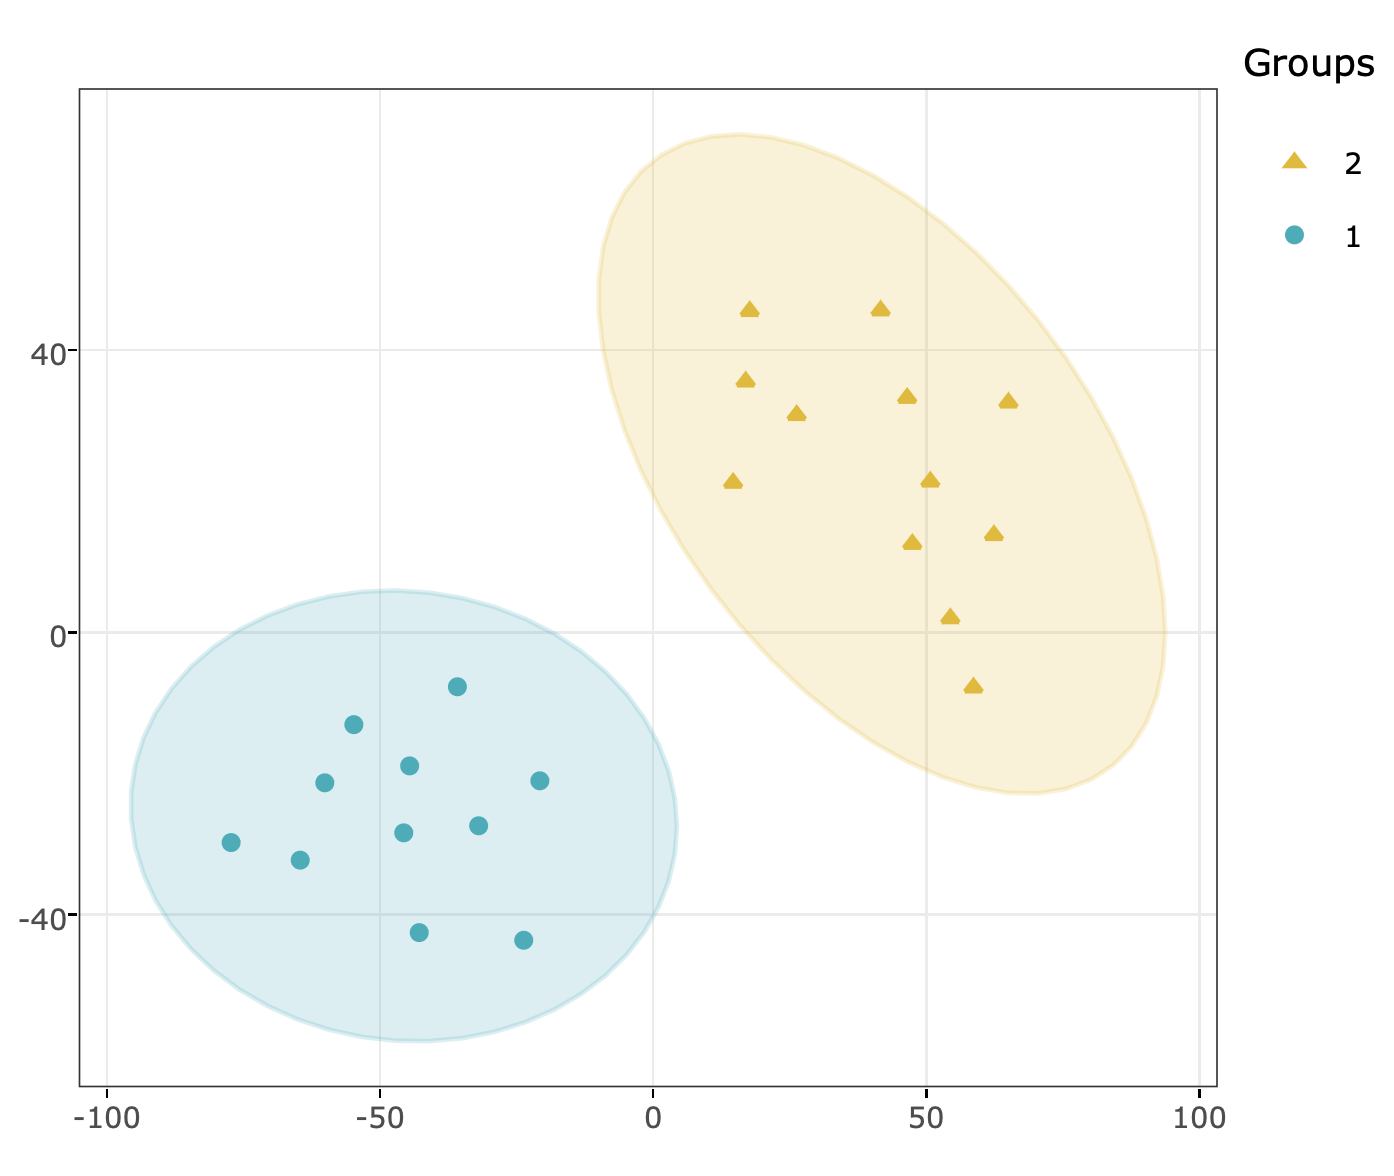
\includegraphics{./image/tsne_plot.png}
\caption{tsne plot}
\end{figure}

\hypertarget{UMAP}{%
\subsection{UMAP}\label{UMAP}}

UMAP (Uniform Manifold Approximation and Projection) using a nonlinear dimensionality reduction method, Manifold learning, which effectively visualizing clusters or groups of data points and their relative proximities. Both tSNE and UMAP are intended to predominantly preserve the local structure that is to group neighbouring data points which certainly delivers a very informative visualization of heterogeneity in the data. The significant difference with t-SNE is scalability, which allows UMAP eliminating the need for applying pre-processing step (such as PCA). Besides, UMAP applies Graph Laplacian for its initialization as tSNE by default implements random initialization. Thus, some people suggest that the key problem of tSNE is the Kullback-Leibler (KL) divergence, which makes UMAP superior over t-SNE. Nevertheless, UMAP's cluster may not good enough for multi-class pattern classification.\textsuperscript{2}

The type of distance metric to find nearest neighbors the size of the local neighborhood (as for the number of neighboring sample points) are set by parameter \texttt{metric} and \texttt{n\_neighbors}. Larger values lead to more global views of the manifold, while smaller values result in more local data being preserved. Generally, values are set in the range of 2 to 100. (default: 15).

\begin{Shaded}
\begin{Highlighting}[]
\CommentTok{# data processing of exp_data}
\NormalTok{exp_transform_table <-}\StringTok{ }\KeywordTok{data_process}\NormalTok{(exp_data, }\DataTypeTok{trans_type=}\StringTok{'log'}\NormalTok{,}
                                    \DataTypeTok{exclude_var_missing=}\OtherTok{TRUE}\NormalTok{,}
                                    \DataTypeTok{missing_pct_limit=}\DecValTok{50}\NormalTok{,}
                                    \DataTypeTok{replace_zero=}\OtherTok{TRUE}\NormalTok{, }\DataTypeTok{replace_NA=}\OtherTok{TRUE}\NormalTok{,}
                                    \DataTypeTok{zero2what=}\StringTok{'min'}\NormalTok{, }\DataTypeTok{xmin=}\FloatTok{0.5}\NormalTok{,}
                                    \DataTypeTok{NA2what=}\StringTok{'min'}\NormalTok{, }\DataTypeTok{ymin=}\FloatTok{0.5}\NormalTok{,}
                                    \DataTypeTok{pct_transform=}\OtherTok{TRUE}\NormalTok{, }\DataTypeTok{centering=}\OtherTok{FALSE}\NormalTok{,}
                                    \DataTypeTok{data_transform=}\OtherTok{TRUE}\NormalTok{, }\DataTypeTok{scaling=}\OtherTok{FALSE}\NormalTok{ )}
\CommentTok{# conduct UMAP}
\NormalTok{UMAP_result <-}\StringTok{ }\KeywordTok{UMAP}\NormalTok{(exp_transform_table, }\DataTypeTok{group_info=}\OtherTok{NULL}\NormalTok{,}
                    \DataTypeTok{sig_feature=}\OtherTok{NULL}\NormalTok{, }\DataTypeTok{n_neighbors=}\DecValTok{15}\NormalTok{,}
                    \DataTypeTok{scale=}\OtherTok{TRUE}\NormalTok{, }\DataTypeTok{metric=}\StringTok{'euclidean'}\NormalTok{, }\DataTypeTok{group_num=}\DecValTok{2}\NormalTok{,}
                    \DataTypeTok{cluster_method=}\StringTok{'kmeans'}\NormalTok{, }\DataTypeTok{var1=}\OtherTok{NULL}\NormalTok{, }\DataTypeTok{var2=}\OtherTok{NULL}\NormalTok{,}
                    \DataTypeTok{insert_ref_group=}\OtherTok{NULL}\NormalTok{, }\DataTypeTok{ref_group=}\OtherTok{NULL}\NormalTok{)}

\CommentTok{# view result: data frame of UMAP data}
\KeywordTok{head}\NormalTok{(UMAP_result[[}\DecValTok{1}\NormalTok{]], }\DecValTok{5}\NormalTok{)}
\end{Highlighting}
\end{Shaded}


  \providecommand{\huxb}[2]{\arrayrulecolor[RGB]{#1}\global\arrayrulewidth=#2pt}
  \providecommand{\huxvb}[2]{\color[RGB]{#1}\vrule width #2pt}
  \providecommand{\huxtpad}[1]{\rule{0pt}{#1}}
  \providecommand{\huxbpad}[1]{\rule[-#1]{0pt}{#1}}

\begin{table}[ht]
\begin{centerbox}
\begin{threeparttable}
 \label{tab:Profiling: dimensionality reduction - UMAP}
\setlength{\tabcolsep}{0pt}
\begin{tabular}{l l l l}


\hhline{>{\huxb{0, 0, 0}{0.4}}->{\huxb{0, 0, 0}{0.4}}->{\huxb{0, 0, 0}{0.4}}->{\huxb{0, 0, 0}{0.4}}-}
\arrayrulecolor{black}

\multicolumn{1}{!{\huxvb{0, 0, 0}{0.4}}l!{\huxvb{0, 0, 0}{0}}}{\huxtpad{6pt + 1em}\raggedright \hspace{6pt} \textbf{sample\_name} \hspace{6pt}\huxbpad{6pt}} &
\multicolumn{1}{l!{\huxvb{0, 0, 0}{0}}}{\huxtpad{6pt + 1em}\raggedright \hspace{6pt} \textbf{group} \hspace{6pt}\huxbpad{6pt}} &
\multicolumn{1}{r!{\huxvb{0, 0, 0}{0}}}{\huxtpad{6pt + 1em}\raggedleft \hspace{6pt} \textbf{UMAP-1} \hspace{6pt}\huxbpad{6pt}} &
\multicolumn{1}{r!{\huxvb{0, 0, 0}{0.4}}}{\huxtpad{6pt + 1em}\raggedleft \hspace{6pt} \textbf{UMAP-2} \hspace{6pt}\huxbpad{6pt}} \tabularnewline[-0.5pt]


\hhline{>{\huxb{0, 0, 0}{0.4}}->{\huxb{0, 0, 0}{0.4}}->{\huxb{0, 0, 0}{0.4}}->{\huxb{0, 0, 0}{0.4}}-}
\arrayrulecolor{black}

\multicolumn{1}{!{\huxvb{0, 0, 0}{0.4}}l!{\huxvb{0, 0, 0}{0}}}{\cellcolor[RGB]{242, 242, 242}\huxtpad{6pt + 1em}\raggedright \hspace{6pt} control\_01 \hspace{6pt}\huxbpad{6pt}} &
\multicolumn{1}{l!{\huxvb{0, 0, 0}{0}}}{\cellcolor[RGB]{242, 242, 242}\huxtpad{6pt + 1em}\raggedright \hspace{6pt} 2 \hspace{6pt}\huxbpad{6pt}} &
\multicolumn{1}{r!{\huxvb{0, 0, 0}{0}}}{\cellcolor[RGB]{242, 242, 242}\huxtpad{6pt + 1em}\raggedleft \hspace{6pt} 0.21\hphantom{0} \hspace{6pt}\huxbpad{6pt}} &
\multicolumn{1}{r!{\huxvb{0, 0, 0}{0.4}}}{\cellcolor[RGB]{242, 242, 242}\huxtpad{6pt + 1em}\raggedleft \hspace{6pt} -0.831 \hspace{6pt}\huxbpad{6pt}} \tabularnewline[-0.5pt]


\hhline{>{\huxb{0, 0, 0}{0.4}}|>{\huxb{0, 0, 0}{0.4}}|}
\arrayrulecolor{black}

\multicolumn{1}{!{\huxvb{0, 0, 0}{0.4}}l!{\huxvb{0, 0, 0}{0}}}{\huxtpad{6pt + 1em}\raggedright \hspace{6pt} control\_02 \hspace{6pt}\huxbpad{6pt}} &
\multicolumn{1}{l!{\huxvb{0, 0, 0}{0}}}{\huxtpad{6pt + 1em}\raggedright \hspace{6pt} 1 \hspace{6pt}\huxbpad{6pt}} &
\multicolumn{1}{r!{\huxvb{0, 0, 0}{0}}}{\huxtpad{6pt + 1em}\raggedleft \hspace{6pt} 0.232 \hspace{6pt}\huxbpad{6pt}} &
\multicolumn{1}{r!{\huxvb{0, 0, 0}{0.4}}}{\huxtpad{6pt + 1em}\raggedleft \hspace{6pt} -0.173 \hspace{6pt}\huxbpad{6pt}} \tabularnewline[-0.5pt]


\hhline{>{\huxb{0, 0, 0}{0.4}}|>{\huxb{0, 0, 0}{0.4}}|}
\arrayrulecolor{black}

\multicolumn{1}{!{\huxvb{0, 0, 0}{0.4}}l!{\huxvb{0, 0, 0}{0}}}{\cellcolor[RGB]{242, 242, 242}\huxtpad{6pt + 1em}\raggedright \hspace{6pt} control\_03 \hspace{6pt}\huxbpad{6pt}} &
\multicolumn{1}{l!{\huxvb{0, 0, 0}{0}}}{\cellcolor[RGB]{242, 242, 242}\huxtpad{6pt + 1em}\raggedright \hspace{6pt} 2 \hspace{6pt}\huxbpad{6pt}} &
\multicolumn{1}{r!{\huxvb{0, 0, 0}{0}}}{\cellcolor[RGB]{242, 242, 242}\huxtpad{6pt + 1em}\raggedleft \hspace{6pt} -1.74\hphantom{0} \hspace{6pt}\huxbpad{6pt}} &
\multicolumn{1}{r!{\huxvb{0, 0, 0}{0.4}}}{\cellcolor[RGB]{242, 242, 242}\huxtpad{6pt + 1em}\raggedleft \hspace{6pt} -0.662 \hspace{6pt}\huxbpad{6pt}} \tabularnewline[-0.5pt]


\hhline{>{\huxb{0, 0, 0}{0.4}}|>{\huxb{0, 0, 0}{0.4}}|}
\arrayrulecolor{black}

\multicolumn{1}{!{\huxvb{0, 0, 0}{0.4}}l!{\huxvb{0, 0, 0}{0}}}{\huxtpad{6pt + 1em}\raggedright \hspace{6pt} control\_04 \hspace{6pt}\huxbpad{6pt}} &
\multicolumn{1}{l!{\huxvb{0, 0, 0}{0}}}{\huxtpad{6pt + 1em}\raggedright \hspace{6pt} 1 \hspace{6pt}\huxbpad{6pt}} &
\multicolumn{1}{r!{\huxvb{0, 0, 0}{0}}}{\huxtpad{6pt + 1em}\raggedleft \hspace{6pt} 0.729 \hspace{6pt}\huxbpad{6pt}} &
\multicolumn{1}{r!{\huxvb{0, 0, 0}{0.4}}}{\huxtpad{6pt + 1em}\raggedleft \hspace{6pt} -0.852 \hspace{6pt}\huxbpad{6pt}} \tabularnewline[-0.5pt]


\hhline{>{\huxb{0, 0, 0}{0.4}}|>{\huxb{0, 0, 0}{0.4}}|}
\arrayrulecolor{black}

\multicolumn{1}{!{\huxvb{0, 0, 0}{0.4}}l!{\huxvb{0, 0, 0}{0}}}{\cellcolor[RGB]{242, 242, 242}\huxtpad{6pt + 1em}\raggedright \hspace{6pt} control\_05 \hspace{6pt}\huxbpad{6pt}} &
\multicolumn{1}{l!{\huxvb{0, 0, 0}{0}}}{\cellcolor[RGB]{242, 242, 242}\huxtpad{6pt + 1em}\raggedright \hspace{6pt} 2 \hspace{6pt}\huxbpad{6pt}} &
\multicolumn{1}{r!{\huxvb{0, 0, 0}{0}}}{\cellcolor[RGB]{242, 242, 242}\huxtpad{6pt + 1em}\raggedleft \hspace{6pt} -0.739 \hspace{6pt}\huxbpad{6pt}} &
\multicolumn{1}{r!{\huxvb{0, 0, 0}{0.4}}}{\cellcolor[RGB]{242, 242, 242}\huxtpad{6pt + 1em}\raggedleft \hspace{6pt} -0.447 \hspace{6pt}\huxbpad{6pt}} \tabularnewline[-0.5pt]


\hhline{>{\huxb{0, 0, 0}{0.4}}->{\huxb{0, 0, 0}{0.4}}->{\huxb{0, 0, 0}{0.4}}->{\huxb{0, 0, 0}{0.4}}-}
\arrayrulecolor{black}
\end{tabular}
\end{threeparttable}\par\end{centerbox}

\end{table}


\begin{Shaded}
\begin{Highlighting}[]
\CommentTok{# view result: UMAP plot}
\NormalTok{UMAP_result[[}\DecValTok{2}\NormalTok{]]   }
\end{Highlighting}
\end{Shaded}

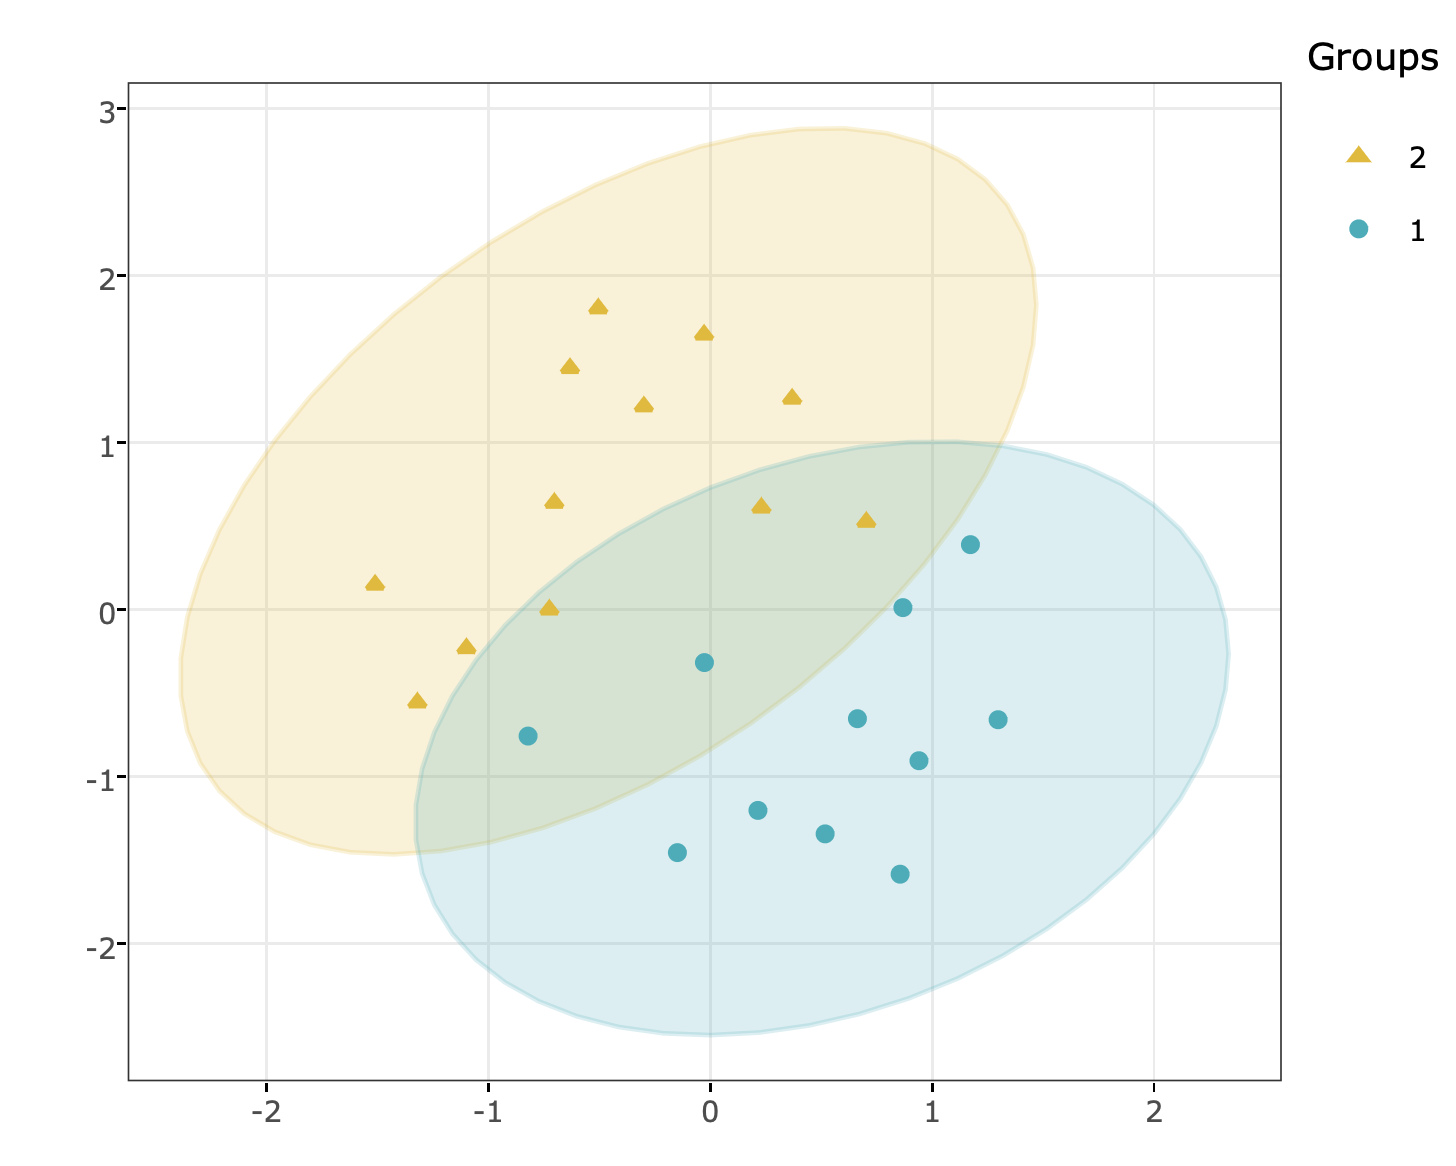
\includegraphics{./image/UMAP_plot.png}

\hypertarget{correlation-heatmap}{%
\section{Correlation heatmap}\label{correlation-heatmap}}

The correlation heatmap illustrates the correlation between samples or lipid species and also depicts the patterns in each group. The correlation is calculated by the method defined by parameter \texttt{corr\_method}, and the correlation coefficient is then clustered depending on method defined by parameter \texttt{distfun} and the distance defined by parameter \texttt{hclustfun}. Two heatmaps will be shown by lipid species and by samples. Please note that if the number of lipids or samples is over 50, the names of lipids/samples will not be shown on the heatmap.

\begin{Shaded}
\begin{Highlighting}[]
\CommentTok{# data processing of exp_data}
\NormalTok{exp_transform <-}\StringTok{ }\KeywordTok{data_process}\NormalTok{(exp_data, }\DataTypeTok{exclude_var_missing=}\OtherTok{TRUE}\NormalTok{,}
                              \DataTypeTok{missing_pct_limit=}\DecValTok{50}\NormalTok{, }\DataTypeTok{replace_zero=}\OtherTok{TRUE}\NormalTok{,}
                              \DataTypeTok{zero2what=}\StringTok{'min'}\NormalTok{, }\DataTypeTok{xmin=}\FloatTok{0.5}\NormalTok{, }\DataTypeTok{replace_NA=}\OtherTok{TRUE}\NormalTok{,}
                              \DataTypeTok{NA2what=}\StringTok{'min'}\NormalTok{, }\DataTypeTok{ymin=}\FloatTok{0.5}\NormalTok{, }\DataTypeTok{pct_transform=}\OtherTok{TRUE}\NormalTok{,}
                              \DataTypeTok{data_transform=}\OtherTok{TRUE}\NormalTok{, }\DataTypeTok{trans_type=}\StringTok{'log'}\NormalTok{,}
                              \DataTypeTok{centering=}\OtherTok{FALSE}\NormalTok{, }\DataTypeTok{scaling=}\OtherTok{FALSE}\NormalTok{)}
\CommentTok{# correlation calculation}
\NormalTok{corr_result <-}\StringTok{ }\KeywordTok{corr_heatmap}\NormalTok{(exp_transform, }\DataTypeTok{corr_method=}\StringTok{"pearson"}\NormalTok{,}
                            \DataTypeTok{distfun=}\StringTok{"maximum"}\NormalTok{, }\DataTypeTok{hclustfun=}\StringTok{"average"}\NormalTok{)}

\CommentTok{# view result: matrix of correlation coefficients           }
\KeywordTok{head}\NormalTok{(corr_result}\OperatorTok{$}\NormalTok{sample_corr_coef[, }\DecValTok{1}\OperatorTok{:}\DecValTok{5}\NormalTok{], }\DecValTok{5}\NormalTok{)}
\CommentTok{##            control_01 control_02 control_03 control_04 control_05}
\CommentTok{## control_01  1.0000000  0.8436678  0.8369328  0.8540800  0.8734609}
\CommentTok{## control_02  0.8436678  1.0000000  0.7457617  0.8255156  0.8040823}
\CommentTok{## control_03  0.8369328  0.7457617  1.0000000  0.7739019  0.7849288}
\CommentTok{## control_04  0.8540800  0.8255156  0.7739019  1.0000000  0.7201342}
\CommentTok{## control_05  0.8734609  0.8040823  0.7849288  0.7201342  1.0000000}
\CommentTok{# view result: matrix of correlation p-value  }
\KeywordTok{head}\NormalTok{(corr_result}\OperatorTok{$}\NormalTok{sample_corr_p[, }\DecValTok{1}\OperatorTok{:}\DecValTok{4}\NormalTok{], }\DecValTok{5}\NormalTok{)}
\CommentTok{##              control_01   control_02   control_03   control_04}
\CommentTok{## control_01 0.000000e+00 2.473172e-48 6.844569e-47 1.056963e-50}
\CommentTok{## control_02 2.473172e-48 0.000000e+00 3.718806e-32 1.367375e-44}
\CommentTok{## control_03 6.844569e-47 3.718806e-32 0.000000e+00 5.897612e-36}
\CommentTok{## control_04 1.056963e-50 1.367375e-44 5.897612e-36 0.000000e+00}
\CommentTok{## control_05 1.203055e-55 1.079608e-40 1.344742e-37 4.167638e-29}
\CommentTok{# view result: matrix of reorder sample correlation}
\KeywordTok{head}\NormalTok{(corr_result}\OperatorTok{$}\NormalTok{reorder_sample_corr_coef[, }\DecValTok{1}\OperatorTok{:}\DecValTok{3}\NormalTok{], }\DecValTok{5}\NormalTok{)}
\CommentTok{##                  hfref_patient_10 hfref_patient_04 hfref_patient_05}
\CommentTok{## hfref_patient_13        0.6976086        0.6809920        0.7187572}
\CommentTok{## hfref_patient_12        0.7310794        0.7062071        0.7171976}
\CommentTok{## hfref_patient_11        0.5647891        0.7577328        0.7851855}
\CommentTok{## hfref_patient_10        1.0000000        0.6060374        0.6578909}
\CommentTok{## hfref_patient_09        0.6871129        0.7057743        0.6171108}
\CommentTok{# view result: matrix of correlation coefficients between lipids}
\KeywordTok{head}\NormalTok{(corr_result}\OperatorTok{$}\NormalTok{lipids_corr_coef[, }\DecValTok{1}\OperatorTok{:}\DecValTok{5}\NormalTok{], }\DecValTok{5}\NormalTok{)}
\CommentTok{##            Cer 38:1;2 Cer 40:1;2 Cer 40:2;2 Cer 42:1;2 Cer 42:2;2}
\CommentTok{## Cer 38:1;2 1.00000000  0.2676729  0.2647730  0.3129075 0.01703923}
\CommentTok{## Cer 40:1;2 0.26767290  1.0000000  0.5201040  0.7863653 0.43877001}
\CommentTok{## Cer 40:2;2 0.26477303  0.5201040  1.0000000  0.4727582 0.42078183}
\CommentTok{## Cer 42:1;2 0.31290745  0.7863653  0.4727582  1.0000000 0.43310999}
\CommentTok{## Cer 42:2;2 0.01703923  0.4387700  0.4207818  0.4331100 1.00000000}
\CommentTok{# view result: matrix of correlation p-value between lipids}
\KeywordTok{head}\NormalTok{(corr_result}\OperatorTok{$}\NormalTok{lipid_corr_p[, }\DecValTok{1}\OperatorTok{:}\DecValTok{4}\NormalTok{], }\DecValTok{5}\NormalTok{)}
\CommentTok{##               Cer 38:1;2   Cer 40:1;2 Cer 40:2;2   Cer 42:1;2}
\CommentTok{## Cer 38:1;2 7.469380e-166 2.169008e-01 0.22211240 1.460114e-01}
\CommentTok{## Cer 40:1;2  2.169008e-01 0.000000e+00 0.01095933 8.635027e-06}
\CommentTok{## Cer 40:2;2  2.221124e-01 1.095933e-02 0.00000000 2.271903e-02}
\CommentTok{## Cer 42:1;2  1.460114e-01 8.635027e-06 0.02271903 0.000000e+00}
\CommentTok{## Cer 42:2;2  9.384919e-01 3.621739e-02 0.04556576 3.897876e-02}
\end{Highlighting}
\end{Shaded}

\begin{Shaded}
\begin{Highlighting}[]
\CommentTok{# view result: sample-sample heatmap}
\NormalTok{corr_result}\OperatorTok{$}\NormalTok{sample_hm  }
\end{Highlighting}
\end{Shaded}

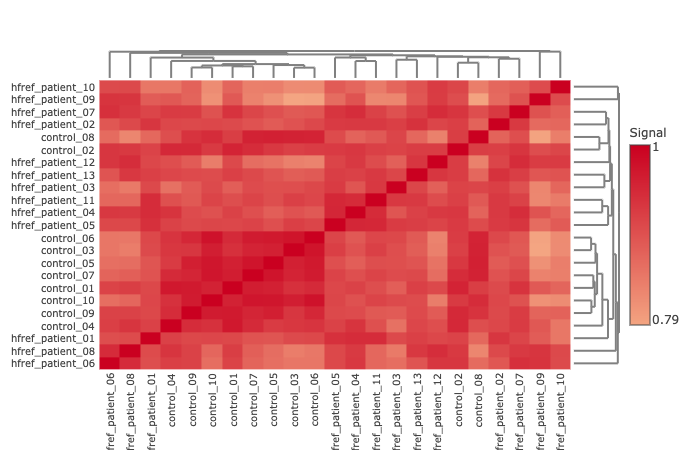
\includegraphics{./image/corr_heatmap_1.png}
The above heatmap reveals sample to sample correlations. Correlations between lipid species are colored from strong positive correlations (red) to no correlation (white).

\begin{Shaded}
\begin{Highlighting}[]
\CommentTok{# view result: lipid-lipid correlations heatmap}
\NormalTok{corr_result}\OperatorTok{$}\NormalTok{lipids_hm}
\end{Highlighting}
\end{Shaded}

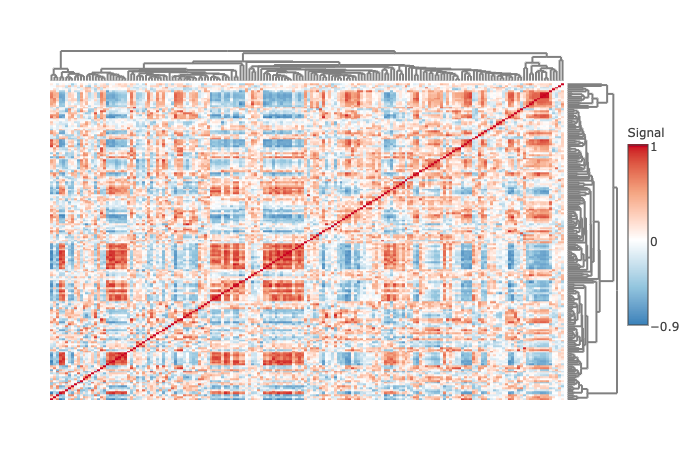
\includegraphics{./image/corr_heatmap_2.png}
The above heatmap illustrates the lipid to lipid correlations. Correlations between lipid species are colored from strong positive correlation (red) to no correlation (white), to negative correlation (blue).

\hypertarget{subsec:pro-char}{%
\section{Lipid characteristics}\label{subsec:pro-char}}

Now, we are going to take a view of lipid expression over specific lipid characteristics. First, lipids are classified by characteristics selected from the `Lipid characteristics' table. Here, we select ``class'' as the selected lipid characteristic. The results will be showed by two plots.

\begin{Shaded}
\begin{Highlighting}[]
\CommentTok{# lipid characteristic}
\NormalTok{char_var <-}\StringTok{ }\KeywordTok{colnames}\NormalTok{(lipid_char_table)[}\OperatorTok{-}\DecValTok{1}\NormalTok{]}
\CommentTok{# calculate lipid expression of selected characteristic}
\NormalTok{compo_result <-}\StringTok{ }\KeywordTok{exp_compo_by_lipidinfo}\NormalTok{(exp_data, lipid_char_table, char_var[}\DecValTok{1}\NormalTok{])}
\end{Highlighting}
\end{Shaded}

\begin{Shaded}
\begin{Highlighting}[]
\CommentTok{# view result: bar plot}
\NormalTok{compo_result}\OperatorTok{$}\NormalTok{p.barplot.p  }
\end{Highlighting}
\end{Shaded}

\begin{figure}
\centering
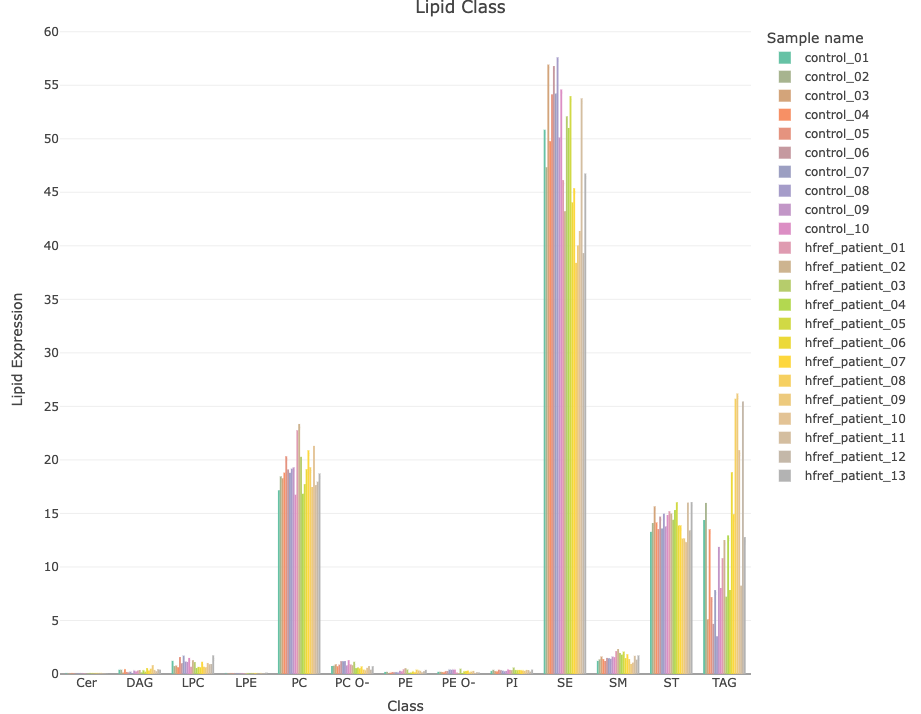
\includegraphics{./image/exp_compo_by_lipidinfo_01.png}
\caption{``Bar plot classified by selected characteristic. The bar plot depicts the expression level of each sample within each group (e.g., PE, PC) of selected characteristics (e.g., class).''}
\end{figure}

\begin{Shaded}
\begin{Highlighting}[]
\CommentTok{# view result: stacked horizontal bar chart}
\NormalTok{compo_result}\OperatorTok{$}\NormalTok{p.compos      }
\end{Highlighting}
\end{Shaded}

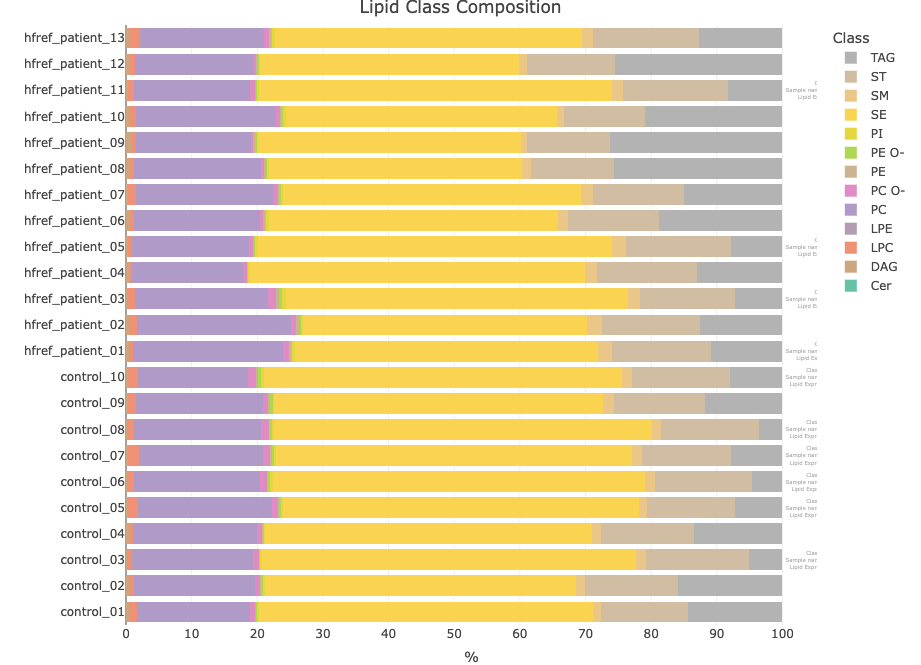
\includegraphics{./image/exp_compo_by_lipidinfo_02.png}
\# Session info

\begin{verbatim}
## R version 4.0.0 (2020-04-24)
## Platform: x86_64-pc-linux-gnu (64-bit)
## Running under: CentOS Linux 7 (Core)
##
## Matrix products: default
## BLAS:   /usr/local/lib64/R/lib/libRblas.so
## LAPACK: /usr/local/lib64/R/lib/libRlapack.so
##
## locale:
##  [1] LC_CTYPE=en_US.UTF-8       LC_NUMERIC=C
##  [3] LC_TIME=en_US.UTF-8        LC_COLLATE=en_US.UTF-8
##  [5] LC_MONETARY=en_US.UTF-8    LC_MESSAGES=en_US.UTF-8
##  [7] LC_PAPER=en_US.UTF-8       LC_NAME=C
##  [9] LC_ADDRESS=C               LC_TELEPHONE=C
## [11] LC_MEASUREMENT=en_US.UTF-8 LC_IDENTIFICATION=C
##
## attached base packages:
## [1] stats     graphics  grDevices utils     datasets  methods   base
##
## other attached packages:
## [1] huxtable_5.4.0   plotly_4.9.4.1   ggplot2_3.3.5    LipidSigR_0.1.0
## [5] BiocStyle_2.16.1
##
## loaded via a namespace (and not attached):
##  [1] httr_1.4.2          tidyr_1.1.4         jsonlite_1.7.2
##  [4] viridisLite_0.4.0   carData_3.0-4       assertthat_0.2.1
##  [7] BiocManager_1.30.16 iheatmapr_0.5.1     cellranger_1.1.0
## [10] yaml_2.2.1          ggrepel_0.9.1       factoextra_1.0.7
## [13] pillar_1.6.3        backports_1.2.1     lattice_0.20-45
## [16] glue_1.4.2          digest_0.6.28       RColorBrewer_1.1-2
## [19] ggsignif_0.6.3      colorspace_2.0-2    htmltools_0.5.2
## [22] Matrix_1.3-4        pkgconfig_2.0.3     broom_0.7.9
## [25] haven_2.4.3         bookdown_0.24       purrr_0.3.4
## [28] scales_1.1.1        webshot_0.5.2       processx_3.5.2
## [31] RSpectra_0.16-0     openxlsx_4.2.4      Rtsne_0.15
## [34] rio_0.5.27          tibble_3.1.4        generics_0.1.0
## [37] farver_2.1.0        car_3.0-11          ellipsis_0.3.2
## [40] ggpubr_0.4.0        withr_2.4.2         fastcluster_1.2.3
## [43] lazyeval_0.2.2      magrittr_2.0.1      crayon_1.4.1
## [46] readxl_1.3.1        evaluate_0.14       ps_1.6.0
## [49] fansi_0.5.0         rstatix_0.7.0       forcats_0.5.1
## [52] foreign_0.8-81      FNN_1.1.3           tools_4.0.0
## [55] data.table_1.14.2   hms_1.1.1           lifecycle_1.0.1
## [58] stringr_1.4.0       munsell_0.5.0       zip_2.2.0
## [61] callr_3.7.0         compiler_4.0.0      rlang_0.4.11
## [64] grid_4.0.0          htmlwidgets_1.5.4   crosstalk_1.1.1
## [67] labeling_0.4.2      rmarkdown_2.11      gtable_0.3.0
## [70] abind_1.4-5         DBI_1.1.1           curl_4.3.2
## [73] R6_2.5.1            knitr_1.34          dplyr_1.0.7
## [76] fastmap_1.1.0       uwot_0.1.10         utf8_1.2.2
## [79] commonmark_1.7      stringi_1.7.4       Rcpp_1.0.7
## [82] vctrs_0.3.8         tidyselect_1.1.1    xfun_0.26
\end{verbatim}

\hypertarget{references}{%
\section*{References}\label{references}}
\addcontentsline{toc}{section}{References}

\hypertarget{refs}{}
\leavevmode\hypertarget{ref-van2008visualizing}{}%
1. Van der Maaten, L. \& Hinton, G. Visualizing data using t-sne. \emph{Journal of machine learning research} \textbf{9,} (2008).

\leavevmode\hypertarget{ref-mcinnes2018umap}{}%
2. McInnes, L., Healy, J. \& Melville, J. Umap: Uniform manifold approximation and projection for dimension reduction. \emph{arXiv preprint arXiv:1802.03426} (2018).


\end{document}
